\documentclass{article}
\usepackage[utf8]{inputenc}
\usepackage{amsthm}
\usepackage{amsmath}
\usepackage{amssymb}
\usepackage{tasks}
\usepackage{tikz}
\usepackage{authblk}
\usepackage{mathtools}

\usetikzlibrary{calc,shapes.geometric, decorations.pathreplacing}

\newtheorem*{definition}{Definition}
\newtheorem*{proposition}{Proposition}
\newtheorem*{lemma}{Lemma}
\newtheorem*{corollary}{Corollary}

\newcommand{\card}[1]{\overline{\overline{#1}}}
\newcommand{\mathbig}[1]{\vcenter{\hbox{\scalebox{1.25}{$#1$}}}}

\newcommand{\R}{\mathbb{R}}
\newcommand{\N}{\mathbb{N}}
\newcommand{\pwrset}{\mathcal{P}}

\newcommand{\B}{\mathcal{B}}
\newcommand{\bcup}{\cup}
\newcommand{\bcap}{\Cap}
\newcommand{\bstar}{^\circledast}
\newcommand{\bcont}{\mathcal{C}^\R}
\newcommand{\bmeasure}{\leq_\mu^\R}

\newcommand{\lang}{\mathcal{L}}
\newcommand{\Vars}{\text{Vars}}
\newcommand{\Pol}{\text{Pol}}


\newcommand{\lcup}{\sqcup}
\newcommand{\lcap}{\sqcap}
\newcommand{\lstar}{^*}
\newcommand{\lpart}{\sqsubseteq}
\newcommand{\lparteq}{\doteq}
\newcommand{\lcont}{C}
\newcommand{\lmeasure}{\preceq}
\newcommand{\lmeasures}{\prec}
\newcommand{\lmeasureeq}{\asymp}

\newcommand{\eqdef}{\stackrel{\text{def}}{=}}
\newcommand{\eqih}{\stackrel{\text{ i.h.}}{=}}
\newcommand{\equivih}{\stackrel{\text{i.h.}}{\leftrightarrow}}

\title{Axiomatization of Some Contact Logics with a Qualitative Measure}
\author{Anguel Nikolov\\{\small supervised by Prof. Tinko Tinchev}}
\affil{Faculty of Mathematics and Informatics \\
  Sofia University ``St. Kliment Ohridski''}
\date{\today}

\begin{document}

\maketitle

\section{Introduction}

The aim of this work is to explore the axiomatization and decidability of the quantifier-free theories of a structure, which arises from a certain kind of geometric objects on the real line. Three relations between these objects are considered: parthood, contact and qualitative measure.

The objects are referred to as polytopes, though they are in fact unions of what may usually be understood by the term. A key property by which they are chosen is that they have a true interior.

The parthood relationship between these objects gives rise to a Boolean algebra and two further relations are considered: contact and qualitative measure.
\section{Notation and Notions}
Described below is the manner in which some established notions are used in this text. Known facts about them are of course implicitly used throughout the text.

\begin{itemize}
\item $\N$ denotes the natural numbers $0, 1, 2, \dots$. $\R$ denotes the real numbers, $\R^+$ denotes the positive real numbers and $\R^+_0$ denotes the non-negative ones.

\item $-\infty$ and $\infty$ are the least and greatest elements of $\R \cup \{-\infty, \infty\}$. They are referred to as infinite and all other real numbers are referred to as finite.

  For the purposes of measure, the $+$ operation over $\R^+_0$ is extended to $\R^+_0 \cup \{\infty\}$ in the usual way:
  \begin{equation*}
    r + \infty \eqdef \infty + r \eqdef \infty \text{, for any } r \in \R^+_0 \cup \{\infty\}
  \end{equation*}

\item $\pwrset(X)$ denotes the set of all subsets of $X$.

\item The cardinality of a set $A$ is denoted by $\card{A}$.

\item $Cl(A)$ and $Int(A)$ denote the closure and interior of the set $A \subseteq \R$ with regard to the standard topology carried by $\R$.

\item A \emph{graph} is an ordered pair $\langle V, E \rangle$ of a finite set of vertices $V$ and a set of edges $E$. Every edge $e \in E$ is a pair of different vertices of $V$, i.e. $e = \{u, v\}$, for some $u \in V$ and $v \in V$, $u \neq v$.

  A \emph{path} from the vertex $u$ to the vertex $w$ in a graph $\langle V, E \rangle$ is a series of vertices $v_1, v_2, \dots, v_n$, such that $u = v_1$, $w = v_n$ and $\{v_i, v_{i+1}\} \in E$, for all $i = 1, 2, \dots, n - 1$.

  A \emph{simple path} in a graph $\langle V, E \rangle$ is a path $v_1, v_2, \dots, v_n$ for which the vertices are distinct, i.e. $i \neq j \rightarrow v_i \neq v_j$, for all $i = 1, 2, \dots, n$ and all $j = 1, 2, \dots, n$.

  A \emph{cycle} in a graph $\langle V, E \rangle$ is a path $v_1, v_2, \dots, v_n, v_1$, such that $v_1, v_2, \dots, v_n$ is a simple path.

  A \emph{connected component} in a graph $\langle V, E \rangle$ is a set of vertices $V' \subseteq V$, such that there exists a path in $\langle V, E \rangle$ from every vertex to every other vertex in $V'$ and there exists no path between any vertex in $V'$ and any vertex in $V \setminus V'$.

  A graph $\langle V, E \rangle$ is \emph{connected} if $V$ is a connected component.

  A \emph{tree} is any connected graph $\langle V, E \rangle$ without cycles.

  A \emph{rooted tree} with root $r$ is a tree $T = \langle V, E \rangle$, where $r \in V$ is singled out. This induces an ordering on the edges in the usual way and determines the children of every vertex $v$, denoted by $Children(T, v)$. There is no implicit ordering on the children of a vertex and when such an ordering is used, it is arbitrary.

  Further, the subtree at vertex $v$, a restriction of $T$ to only the descendants of $v$ is a rooted tree with root $v$, denoted by $SubTree(T, v)$.

\item $\sum_{x \in A}x$ denotes the sum of the elements of $A$ and is equal to $0$ if $A = \emptyset$.
\end{itemize}

\section{Language}
This section describes the language, whose semantics will be considered in a couple of contexts.

\begin{definition}[Language]
  $\lang$ denotes the first-order language with equality of only quantifier-free formulas, containing the following non-logical symbols:
\begin{itemize}
  \item predicate symbols:
  \begin{itemize}
  \item binary infix $\lpart$: parthood
  \item binary infix $\lmeasure$: measure comparison
  \item binary prefix $\lcont$: contact
  \end{itemize}
  \item function symbols:
  \begin{itemize}
  \item binary infix function $\lcup$: union
  \item binary infix function $\lcap$: intersection
  \item unary postfix function $\lstar$: complement
  \end{itemize}
  \item constant symbols:
  \begin{itemize}
  \item $0$: empty polytope
  \item $1$: universe
  \end{itemize}
\end{itemize}

The logical symbols $\land$ and $\lnot$ are used in the typical way. The set of individual variables is denoted by $\Vars$. The symbol for formal equality is $\lparteq$.

The following abbreviations will be used for any terms $\tau_1$ and $\tau_2$:
\begin{itemize}
\item $\tau_1 \lmeasureeq \tau_2$ for $\tau_1 \lmeasure \tau_2 \land \tau_2 \lmeasure \tau_1$
\item $\tau_1 \lmeasures \tau_2$ for $\lnot (\tau_2 \lmeasure \tau_1)$
\end{itemize}
and for any formulas $\phi$ and $\psi$:
\begin{itemize}
\item $\phi \lor \psi$ for $\lnot(\phi \land \psi)$
\item $\phi \Rightarrow \psi$ for $\lnot\phi \lor \psi$
\item $\phi \Leftrightarrow \psi$ for $(\phi \Rightarrow \psi) \land (\psi \Rightarrow \phi)$
\item $\top$ for $\phi \lor \lnot \phi$
\item $\bot$ for $\phi \land \lnot \phi$
\end{itemize}
\end{definition}

\section{Semantics}

Though the aim is to interpret the language on the real line, other structures will also be needed. It is useful fix their common semantics, which are defined below in the expected way.

Let $\B$ be a Boolean algebra with carrier $B$ and $\mathcal{C}$ and $\mathcal{M}$ be relations over $B$. Let $S = \langle \B, \mathcal{C}, \mathcal{M} \rangle$.

\begin{definition}[Value of a Term in $S = \langle \B, \mathcal{C}, \mathcal{M} \rangle$]
  Let $v: \Vars \rightarrow B$. $v$ is implicitly extended to be defined for all terms of $\lang$ in the following structurally recursive way:
  \begin{itemize}
  \item $v(0)$ is the zero of $\B$
  \item $v(1)$ is the unit of $\B$
  \item $v(\tau_1 \lstar)$ is the complement of $v(\tau_1)$ in $\B$,
  \item $v(\tau_1 \lcup \tau_2)$ is the join of $v(\tau_1)$ and $v(\tau_2)$ in $\B$,
  \item $v(\tau_1 \lcap \tau_2)$ is the meet of $v(\tau_1)$ and $v(\tau_2)$ in $\B$,
  \end{itemize}
for any terms $\tau_1$ and $\tau_2$ of $\lang$.

\end{definition}

\begin{definition}[Validity of a Formula in $S = \langle \B, \mathcal{C}, \mathcal{M} \rangle$]
  Again, let $v: \Vars \rightarrow B$. Validity of a formula $\phi$ in $S$ with valuation $v$ is denoted by $\langle S, v \rangle \models \phi$ and defined over atomic formulas like so:
  \begin{itemize}
  \item $\langle S, v \rangle \models \tau_1 \lpart \tau_2 \leftrightarrow v(\tau_1)$ is less than or equal to $v(\tau_2)$ in $\B$,
  \item $\langle S, v \rangle \models \lcont(\tau_1, \tau_2) \leftrightarrow \mathcal{C}(v(\tau_1), v(\tau_2))$,
  \item $\langle S, v \rangle \models \tau_1 \lmeasure \tau_2 \leftrightarrow \mathcal{M}(v(\tau_1), v(\tau_2))$,
  \end{itemize}
  for any terms $\tau_1$ and $\tau_2$ of $\lang$. For complex formulas, the extension is done in the usual way:
  \begin{itemize}
  \item $\langle S, v \rangle \models \top$ and $\langle S, v \rangle \not \models \bot$,
  \item $\langle S, v \rangle \models \lnot \phi \leftrightarrow \langle S, v \rangle \not\models \phi$,
  \item $\langle S, v \rangle \models \phi \land \psi \leftrightarrow \langle S, v \rangle \models \phi$ and $\langle S, v \rangle \models \psi$,
  \item $\langle S, v \rangle \models \phi \lor \psi \leftrightarrow$ at least one of  $\langle S, v \rangle \models \phi$ and $\langle S, v \rangle \models \psi$ holds,
  \end{itemize}
  where $\phi$ and $\psi$ are (quantifier-free) formulas of $\lang$.

  If $\langle S, v \rangle \models \phi$ for all $v: \Vars \rightarrow B$, then $\phi$ is valid in $S$, denoted by $S \models \phi$.

  If there exists $v: \Vars \rightarrow B$ such that $\langle S, v \rangle \models \phi$, then $\phi$ is satisfiable.
\end{definition}

\subsection{Polytopes on the Real Line}

A specific kind of objects will be considered: finite unions of closed, potentially infinite, intervals on the real line. These are defined below, along with the interpretation operations and properties with which the language is concerned.

\begin{definition}[Basis Polytope]
  For any $m$, $n \in \R$ such that $m < n$, the intervals $[m, n]$, $(-\infty, m]$, $[m, \infty)$ and $(-\infty, \infty)$ are called \emph{basis polytopes}. The set of all basis polytopes is $Bas(\R)$.

      In the basis polytopes listed above, $m$ and $-\infty$ are left endpoints and $n$ and $\infty$ are right endpoints.
\end{definition}

\begin{proposition}
  For any two basis polytopes $b_1$ and $b_2$, if $b_1 \cap b_2 \neq \emptyset$, then $b_1 \cup b_2$ is a basis polytope.
\end{proposition}

\begin{definition}[Polytope]
For any finite set of basis polytopes $C \subseteq Bas(\R)$, $\bigcup C$ is called a \emph{polytope}. The set of all polytopes is denoted by $\Pol(\R)$.
\end{definition}
Remark that for $C = \emptyset$, the empty set is also a polytope.

\begin{definition}(Standard Representation)
If the set of basis polytopes is disjoint, i.e. $C \subseteq Bas(\R)$ and $(\forall b_1 \in C)(\forall b_2 \in C)(b_1 \neq b_2 \rightarrow b_1 \cap b_2 = 0)$, then $C$ is called a \emph{standard representation} of the polytope $\bigcup C$.
\end{definition}

\begin{proposition}
Every polytope has exactly one standard representation.
\end{proposition}
\begin{proof}
  Let $p$ be an arbitrary polytope. Let $A$ be the set of representations of $p$, i.e. $A \eqdef \{\, C \mid C \subseteq Bas(\R) \text{, } C \text{ is finite and } \bigcup C = p\}$. Since $p$ is a polytope, $A \neq \emptyset$. Let $C'$ be any element of $A$ that has the least number of elements, i.e. $(\forall C \in A)(\card{C'} \leq \card{C})$.

  Let $b_1 \in C'$, $b_2 \in C'$ and $b_1 \neq b_2$. Suppose for the sake of contradiction that $b_1 \cap b_2 \neq \emptyset$. Then, $b_1 \cup b_2 \in Bas(\R)$. Let $D \eqdef C' \cup \{b_1 \cup b_2\} \setminus \{b_1, b_2\}$. $\bigcup D = \bigcup C'$, so $D \in A$ and $\card{D} < \card{C'}$, a contradiction. Thus, the elements of $C'$ are non-intersecting, so $C'$ is a standard representation of $p$.

  Suppose $C''$ is an arbitrary standard representation of $p$. To show that $C'' \subseteq C'$, let $b'' \in C''$ be arbitrary. Fix some $x \in b''$. Then $x \in \bigcup C'' = \bigcup C'$, so let $b_1' \in C'$, such that $x \in b_1'$. Let $y \in b''$ be arbitrary, such that $y \neq x$. Just as for $x$, let $y \in b_2' \in C'$.

  \begin{figure}[ht]
    \centering
    \begin{tikzpicture}
      \node [draw=none] (a) at (-3, -1) {};
      \node [draw=none] (b) at (3, -1) {};
      \draw (-3,-1) -- node[below] {$b''$} (3,-1);
      \node [draw=none] (c) at (-4, 0) {};
      \node [draw=none] (d) at (-1, 0) {};
      \draw (-4,0) -- node[above] {$b_1'$}  (-1,0);
      \node [draw=none] (e) at (1, 0) {};
      \node [draw=none] (f) at (4, 0) {};
      \draw (1,0) -- node[above] {$b_2'$} (4,0);

      \draw [dashed] (-2, 0) -- node[right] {$x$} (-2, -1);
      \draw [dashed] (2, 0) -- node[right] {$y$} (2, -1);

      \foreach \n in {a, b, c, d, e, f}
               {
                 \draw ($ (\n) + (0, +2pt) $) -- ($ (\n) - (0, 2pt) $);
               }
    \end{tikzpicture}
  \end{figure}
  Suppose for the sake of contradiction that $b_1' \neq b_2'$. Without loss of generality, let $x < y$. $[x, y] \subseteq b''$, whence $[x, y] \subseteq \bigcup C'' = p$. Consider the merger of the two intervals and the points between them $b' \eqdef b_1' \cup [x, y] \cup b_2' \in Bas(\R)$ and $C''' \eqdef C' \cup \{b'\} \setminus \{b_1', b_2'\}$. Given that $b' \subseteq p$, $b_1' \subseteq b'$ and $b_2' \subseteq b'$, it follows that $C''' \in A$ and $\card{C'''} < \card{C'}$, a contradiction. Thus, $y \in b_1'$, for any $y \in b''$, so $b'' \subseteq b_1'$.

  Again, for the sake of contradiction, let $b_1' \not \subseteq b''$. Then $b'' \neq (-\infty, \infty)$, so $b''$ has at least one finite endpoint which is also different from the corresponding endpoint of $b_1'$. Without loss of generality, let that endpoint be the left endpoint $m \in \R$. Let the left endpoint of $b_1'$ be $n$, where potentially $n = -\infty$. Let $d$ denote the interval $[n, m)$ if $n \neq -\infty$ or $(-\infty, m)$ otherwise. $d \subseteq b_1' \setminus b''$, so $d \subseteq p$.
\begin{figure}[ht]
    \centering
    \begin{tikzpicture}
      \node [draw=none,label=below:$m$] (a) at (-3, -1) {};
      \node [draw=none] (b) at (3, -1) {};
      \draw (-3,-1) -- node[below] {$b''$} (3,-1);
      \node [draw=none,label=below:$n$] (c) at (-4, 0) {};
      \node [draw=none] (d) at (4, 0) {};
      \draw (-4,0) -- node[above] {$b_1'$}  (4,0);

      \draw [dashed] (-4, -1) -- node[below] {$d$} (-3, -1);

      \foreach \n in {a, b, c, d}
               {
                 \draw ($ (\n) + (0, +2pt) $) -- ($ (\n) - (0, 2pt) $);
               }
    \end{tikzpicture}
\end{figure}

    Therefore, there must be other basis polytopes in $C''$ that contain the elements of $d$. Since there are finitely many basis polytopes in $C''$, let $b_0''$ be the basis polytope with the greatest right endpoint among the elements of $C''$, which contain elements of $d$. Let $m_0$ be that right endpoint of $b_0''$.

    If $m \leq m_0$, then then $m \in b_0'' \cap b''$ and $C''$ does not consist of non-intersecting basis polytopes. If $m_0 < m$, then $(m_0 + m)/2 \not \in \bigcup C'' = p$, but $(m_0+m)/2 \in b_1' \subseteq \bigcup C' = p$. In both cases, there is a contradiction, which means that $b_1' \subseteq b''$, which combined with $b'' \subseteq b_1'$ yields $b'' = b_1'$.

  Therefore, for any $b'' \in C''$, it holds that $b'' \in C'$, i.e. $C'' \subseteq C'$. $C'$ has the least cardinality in $A$ and $C'' \in A$, so $C''$ has the same finite cardinality and is a subset of $C'$. Therefore $C'' = C'$ which means any standard representation of $p$ is equal to $C'$.
\end{proof}

\begin{definition}[Polytope Operations]
For any polytopes $p$ and $q$, we define the following operations as modifications of intersection and complement:
\begin{itemize}
  \item $p \bcap q \eqdef Cl(Int(p \cap q))$;
  \item $p \bstar \eqdef Cl(\R \setminus p) $.
\end{itemize}
The union operation $p \bcup q$ will be considered in the same context, though no modification is needed.
\end{definition}

\begin{proposition}
$\Pol(\R)$ forms a Boolean algebra with
  \begin{itemize}
  \item $\subseteq$ for Boolean inequality,
  \item $\bcap$ for meet,
  \item $\bcup$ for join,
  \item $\bstar$ for complement,
  \item $\emptyset$ for the zero and
  \item $\R$ for the unit.
\end{itemize}
This algebra will be denoted by $\B^\R$.
\end{proposition}
\begin{proof}
  The regularly closed subsets of $\R$ ($A \subseteq \R$ and $Cl(Int(A)) = A$) form a Boolean algebra with the interpretation given above (TODO: cite Halmos or Tarski).

  Since basis polytopes are regular closed sets and the algebra is closed under union, polytopes are also regular closed sets.

  Let $r$ be an arbitrary polytope and $C_r$ be its standard representation. Then, $\R \setminus \bigcup C_r$ can be seen to be a union of non-empty, non-intersecting open intervals, with different, potentially infinite endpoints. Given this, the closure of $\R \setminus \bigcup C_r$ yields a union of the same intervals, but closed, i.e. a union of basis intervals. In other words, $r\bstar$ is a polytope.

  Clearly, $p \cup q$ is a polytope for arbitrary polytopes $p$ and $q$, since a union of unions is a union. Applying the De Morgan law in the Boolean algebra of regular closed sets, $p \bcap q = (p\bstar \cup q\bstar)\bstar$. Therefore, since $r\bstar$ is a polytope for any polytope $r$, then $p \bcap q$ is also a polytope.

  Since all of the three operations preserve polytopes, $\B^\R$ is a subalgebra of the algebra of all regular closed sets and therefore a Boolean algebra.
\end{proof}

\begin{proposition}
  $\B^\R$ is atomless.
\end{proposition}
\begin{proof}
  Let $p \neq \emptyset$ be a polytope and $C_p$ be the standard representation of $p$. $C_p \neq \emptyset$, so let $b \in C_p$. Consider any $x \in b$ and $y \in b$, such that $x < y$ and $x$ and $y$ are not endpoints. $[x, y] \neq \emptyset$ is a polytope and $[x, y] \subsetneq p$.
\end{proof}

\begin{proposition}
  $\B^\R$ is not $\sigma$-complete.
\end{proposition}
\begin{proof}
  Consider the countably many polytopes $[2n, 2n+1]$, for each natural number $n$. Their join is the set $[0, 1] \cup [2, 3] \cup [4, 5] \cup \dots$.

  Suppose for the sake of contradiction that this set is a polytope $p$. Then $p$ is a finite union of a basis polytopes $C$, $p = \bigcup C$. Clearly, $C \neq \emptyset$.

  If $[m, \infty) \in C$ for some $m$, then let $o > m$ be the least odd natural number, greater than $m$. $o + \frac{1}{2} \in [m, \infty)$, but $o + \frac{1}{2} \not \in [0, 1] \cup [2, 3] \cup [4, 5] \cup \dots$. Therefore, $[m, \infty) \not \in C$ for any $m$. Similarly, $(-\infty, \infty) \not \in C$, since e.g. $1\frac{1}{2} \not \in p$.

        Let
        \[
        R \eqdef \{r \mid (\exists l \in \R)([l, r] \in C) \text{ or } (-\infty, r] \in C\}
        \]
        Since $C$ is finite, $R$ is finite and there is a greatest element in $R$. Let $o'$ be the least natural number, greater than $\max R$. $o' \not \in \bigcup C$, yet $o' \in [0, 1] \cup [2, 3] \cup [4, 5] \cup \dots$, a contradiction.
\end{proof}

\begin{definition}[Line Contact]
Two polytopes $p$ and $q$ are \emph{in contact} if $p \cap q \neq \emptyset$. This is denoted by $\bcont(p, q)$.
\end{definition}

\begin{definition}[Polytope Measure]
  The function $\mu^\R:\Pol(\R) \rightarrow \R^+_0 \cup \{\infty\}$ defined below is called the \emph{polytope measure}. For a basis polytope of the kind $[m, n]$, where $m \in \R$, $n \in \R$ and $m < n$,
  \[\mu^\R([m, n]) = n - m.\]
  For a basis polytope $b$ of the kind $(-\infty, m]$, $[m, \infty)$ or $(-\infty, \infty)$, where $m \in \R$,
      \[\mu^\R(b) \eqdef \infty.\]
      For a polytope $p$ with standard representation $C_p$,
      \[\mu^\R(p) \eqdef \sum_{\mathclap{b \in C_p}} \mu^\R(b).\]

The \emph{qualitative measure relation induced by} $\mu^\R$ is defined
\begin{equation*}
  p \bmeasure q \leftrightarrow \mu^\R(p) \leq \mu^\R(q),
\end{equation*}
  for any $p, q \in \Pol(\R)$.
\end{definition}

Note that the polytope measure defined above is in fact a restriction of the Lebesgue measure on $\R$.

However, for a basis polytope $b$, $\mu^\R(b) > 0$, which demonstrates the following proposition.
\begin{proposition}
The only polytope with measure $0$ is $\emptyset$.
\end{proposition}
\begin{proof}
  Let $p$ be a polytope, such that $\mu^\R(p) = 0$ and $C_p$ is its standard representation. $\sum_{b \in C_p} \mu^\R(b) = 0$. Since the summands are strictly positive, there must be none of them. Therefore, $C_p = \emptyset$ and $p = \emptyset$.
\end{proof}

\begin{proposition}
  $\mu^\R$ is a $\sigma$-additive measure in $\B^\R$, i.e. for any sequence of mutually disjoint polytopes $\{p_i\}_{i \in \N}$, $(\forall i \in \N)(\forall j \in \N)(i \neq j \rightarrow p_i \bcap p_j = \emptyset)$, such that $\bigcup_{i \in \N}p_i \in \Pol(\R)$
  \[\mu^\R\left(\bigcup_{i \in \N}p_i\right) = \sum_{i \in \N} \mu^\R(p_i).\]
\end{proposition}
\begin{proof}
  Let $p$ and $q$ be two polytopes with standard representations $C_p$ and $C_q$, such that $p \bcap q = \emptyset$.
  \[p \cap q = \bigcup_{\mathclap{b \in C_p}}b \cap \bigcup_{\mathclap{b \in C_q}}b = \bigcup_{\mathclap{\substack{b_p \in C_p\\b_q \in C_q}}}b_p \cap b_q\]
  Observe that the intersection of any two basis polytopes is either a basis polytope, $\emptyset$ or a singleton. If in the sum above $b_p \cap b_q$ is a basis polytope $b$, then since $Cl(Int(b)) = b$, at the very least $b \subseteq Cl(Int(p \cap q)) = \emptyset$, which is impossible. Thus, $p \cap q$ is a finite union of singletons and is therefore finite.

  Returning to the sequence $\{p_i\}_{i \in \N}$,
  \[
  \bigcup_{i \in \N}p_i = \bigcup_{i \in \N}\left(p_i \setminus \bigcup_{\substack{j \in \N\\j \neq i}}p_i \cap p_j \right) \cup \bigcup_{\substack{i \in \N \\ j \in \N\\i \neq j}}p_i \cap p_j
  \]
  The right hand side of the equation above is a union of disjoint sets. Using the $\sigma$-additivity of the Lebesgue measure on $\R$, this yields
  \[
  \mu^L\left(\bigcup_{i \in \N}p_i\right) = \sum_{i \in \N}\left(\mu^L(p_i) - \mu^L\left(\bigcup_{\substack{j \in \N\\j \neq i}}p_i \cap p_j\right) \right) + \mu^L\left(\bigcup_{\substack{i \in \N \\ j \in \N\\i \neq j}}p_i \cap p_j\right)
  \]
  where $\mu^L$ is the Lebesgue measure on $\R$. Since $p_i \cap p_j$ is finite for all $i,j \in \N$, $i \neq j$, it follows that $\bigcup_{\substack{j \in \N\\j \neq i}}p_i \cap p_j$ is countable for any $i \in \N$ and that $\bigcup_{\substack{i \in \N \\ j \in \N\\i \neq j}}p_i \cap p_j$ is countable and therefore they both have Lebesgue measures of $0$. Using this,
  \[
  \mu^L\left(\bigcup_{i \in \N}p_i\right) = \sum_{i \in \N}\mu^L(p_i)
  \]
  is obtained. Since the polytope measure is a restriction of the Lebesgue measure and $\bigcup_{i \in \N}p_i$ is a polytope,
  \[
  \mu^\R\left(\bigcup_{i \in \N}p_i\right) = \sum_{i \in \N}\mu^\R(p_i)
  \]
  is obtained.
\end{proof}

\begin{proposition}
 Every non-zero polytope has an arbitrary small non-zero subpolytope.
\end{proposition}
\begin{proof}
The statement is clearly true for any basis polytope and any non-zero polytope is a union of a non-empty set of basis polytopes.
\end{proof}

Given the definition of $\B^\R$, polytope measure and contact above, the structure on the real line is defined directly:

\begin{definition}[Real Line Structure]
  \begin{equation*}
    S^\R \eqdef \langle \B^\R, \bcont, \bmeasure \rangle
  \end{equation*}
\end{definition}

\subsection{Relational Structures}
In order to find appropriate value functions for a well chosen kind of formulas, an abstract model for those formulas will be needed. It is quite generic, yet it turns out to be transformable into an equivalent real line model, given some constraints.

Let $W$ be a finite set and $\B^W$ be the Boolean algebra of all subsets of $W$. Let $\kappa$ be an arbitrary symmetric and reflexive relation over $W$ and let $\mu: W \rightarrow \R^+ \cup \{\infty\}$.

Let $\mathcal{C}^\kappa$ be the relation over $\pwrset(W)$ defined as
\begin{equation*}
  \mathcal{C}^\kappa(a, b) \leftrightarrow (\exists i \in a)(\exists j \in b)(\langle i, j \rangle \in \kappa)
\end{equation*}
Let $\mu$ be implicitly extended to be defined on $\pwrset(W)$ in the following way:
\begin{equation*}
  \mu(a) \eqdef \sum_{i \in a}\mu(i)
\end{equation*}
And finally, let $\leq_\mu$ be the relation over $\pwrset(W)$:
\begin{equation*}
  a \leq_\mu b \leftrightarrow \mu(a) \leq \mu(b),
\end{equation*}
for all $a$, $b \subseteq W$.
\begin{definition}[Relational Structure]
$\langle \B^W, \mathcal{C}^\kappa, \leq_\mu \rangle$ is called the \emph{relational structure for $W$, $\kappa$ and $\mu$}.
\end{definition}

\subsubsection{Converting to a Real Line Structure}
Relational models for formulas are useful because they can be converted to real line models under certain conditions.
\begin{definition}[Contact Graph]
  Let $S = \langle \B^W, \mathcal{C}^\kappa, \leq_\mu \rangle$ be a relational structure. Let $E$ denote the set of pairs of different vertices in $\kappa$, but unordered: $E \eqdef \{\, \{i, j\} \mid \langle i, j \rangle \in \kappa$ \& $i \neq j \,\}$. Note that since $\kappa$ is reflexive and symmetric, no information is lost when obtaining $E$ from $\kappa$.
  The graph $\langle W, E \rangle$ is called the \emph{contact graph of $S$} and  denoted by $Gr(S)$.
\end{definition}
\begin{definition}[Convertible Relational Structure]
Let $S = \langle \B^W, \mathcal{C}^\kappa, \leq_\mu \rangle$ be a relational structure and suppose that the following constraints hold:
\begin{itemize}
\item $Gr(S)$ is connected and
\item there are exactly two elements of $W$ with infinite values for $\mu$, i.e. there exist $i \in W$ and $j \in W$, $i \neq j$ such that:
  \begin{equation*}
    \mu(i) = \mu(j) = \infty \text{ and } (\forall k \in W \setminus \{i, j\})(\mu(k) \in \R^+).
  \end{equation*}
\end{itemize}
Then, $S$ is called a \emph{convertible relational structure}.
\end{definition}

Although a valuation is an infinite object, any given formula contains a finite number of variables. Therefore, only a finite part of the valuation is relevant to the truth value of that formula. The effective construction of a valuation as discussed below is possible because the valuation will always be considered in the context of a formula and will therefore be encodable by a finite object.

\begin{lemma}[Untying]
  Let $S = \langle \B^W, \mathcal{C}^\kappa, \leq_\mu \rangle$ be a convertible relational structure and $v$ be a valuation. Suppose $Gr(S)$ is not a tree.
  Then, there is a procedure to effectively construct a convertible relational structure $S'$ and a valuation $v'$ for $S'$ such that:
  \begin{itemize}
  \item $Gr(S')$ has one vertex more and the same number of edges and
  \item for any formula $\phi$ in $\lang$, $\langle S, v \rangle \models \phi \leftrightarrow \langle S', v' \rangle \models \phi$.
  \end{itemize}
\end{lemma}
\begin{proof}
  Given that $Gr(S)$ is not a tree, yet is connected, it must contain at least one cycle. A cycle can be effectively found using a depth-first search. Let $\pi$ be such a cycle.

  Let $i$ and $j$ be any two consecutive vertices in $\pi$ such that $\mu(i) \neq \infty$. This requirement is always achievable, since there are at least three vertices in a cycle and only two vertices with infinite values for $\mu$ in a convertible relational structure. Therefore, there will be at least one vertex with a finite value for $\mu$ in any cycle.

  The aim is to disconnect $\pi$ by removing the edge between $i$ and $j$. In order to achieve that, intuitively, the portion of $i$ which is in contact only with $j$ will be separated out into a separate atomic object, $i'$, having half the measure.

\begin{figure}[ht]
    \centering
    \begin{minipage}{0.45\textwidth}
      \centering
      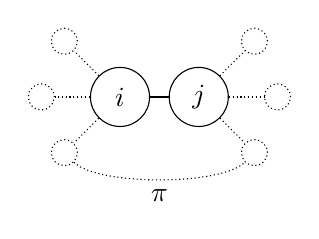
\begin{tikzpicture}[main/.style = {draw, circle, minimum size=.75cm},
          small/.style = {draw, densely dotted, circle, minimum size=.25cm},
          dedge/.style = {densely dotted}]
        \node[main] (i) {$i$};
        \node[main] (j) [right of=i] {$j$};
        \node[small] (i1) [below left of=i] {};
        \node[small] (i2) [above left of=i] {};
        \node[small] (i3) [left of=i] {};
        \node[small] (j1) [below right of=j] {};
        \node[small] (j2) [above right of=j] {};
        \node[small] (j3) [right of=j] {};
        \draw (i) -- (j);
        \foreach \n in {i1, i2, i3}
                 {
                   \draw[dedge] (i) -- (\n);
                 }
        \foreach \n in {j1, j2, j3}
                 {
                   \draw[dedge] (j) -- (\n);
                 }
        \draw[dedge] (i1) to [out=315, in=225, looseness=.5] node[midway, below] {$\pi$} (j1);
      \end{tikzpicture}
    \end{minipage}$\rightsquigarrow$
    \begin{minipage}{0.45\textwidth}
      \centering
      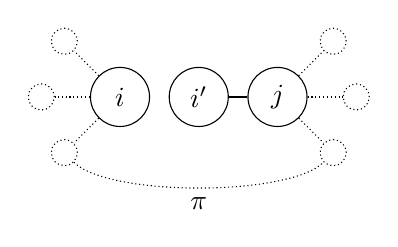
\begin{tikzpicture}[main/.style = {draw, circle, minimum size=.75cm},
          small/.style = {draw, densely dotted, circle, minimum size=.25cm},
          dedge/.style = {densely dotted}]
        \node[main] (i) {$i$};
        \node[main] (i') [right of=i] {$i'$};
        \node[main] (j) [right of=i'] {$j$};
        \node[small] (i1) [below left of=i] {};
        \node[small] (i2) [above left of=i] {};
        \node[small] (i3) [left of=i] {};
        \node[small] (j1) [below right of=j] {};
        \node[small] (j2) [above right of=j] {};
        \node[small] (j3) [right of=j] {};
        \draw (i') -- (j);
        \foreach \n in {i1, i2, i3}
                 {
                   \draw[dedge] (i) -- (\n);
                 }
        \foreach \n in {j1, j2, j3}
                 {
                   \draw[dedge] (j) -- (\n);
                 }
%        \draw[dedge] (i1)  (j1);
        \draw[dedge] (i1) to [out=315, in=225, looseness=.5] node[midway, below] {$\pi$} (j1);
      \end{tikzpicture}
    \end{minipage}
\end{figure}

  Let $i' \not \in W$ and let:
\begin{align*}
W' &\eqdef W \cup \{i'\} \\
\kappa' &\eqdef (\kappa \setminus \{\langle i, j \rangle, \langle j, i \rangle\}) \cup \{\langle i', j \rangle, \langle j, i' \rangle, \langle i', i' \rangle\} \\
\mu'(k) &\eqdef \begin{cases}
\mu(k)           & \text{if $k \not \in \{i, i'\}$} \\
\mu(i) / 2       & \text{otherwise}
\end{cases}\text{, for any } k \in W'. \\
S' &\eqdef \langle \B^{W'}, \mathcal{C}^{\kappa'}, \leq_{\mu'} \rangle \\
v'(x) &\eqdef \begin{cases}
  v(x) \cup \{i'\} & \text{if } i \in v(x) \\
  v(x)             & \text{otherwise}
\end{cases}\text{, for any } x \in \Vars.
\end{align*}

Note that $S'$ and $v'$ are defined in a constructive way. The procedure consists of copying $S$ and $v$, except for a small number of changes, not depending on the size of $S$.

It is directly clear that $S'$ is a relational structure. Compared to $S$, there is one more vertex in $Gr(S')$ and the same number of edges ($\{i, j\}$ is removed, $\{i', j\}$ is added).

Any path between two vertices in $Gr(S)$ corresponds to a path in $Gr(S')$, by potentially substituting the edge $\{i, j\}$ for the detour path along $\pi$. Therefore, all vertices in $W$ are connected in $Gr(S')$. $i'$ is connected to $i$ and from there to the rest of $W$ as well, so $Gr(S')$ is connected.

$\mu'$ has the same values as $\mu$ over all elements of $W'$, except $i$ and $i'$, where it's values are finite. Therefore, the same two elements of $W'$ that have infinite values for $\mu$, also have infinite values for $\mu'$ and no others.

Thus, $S'$ is a convertible relational structure.

Now follows a proof by induction on the construction of the terms in $\lang$, that
\begin{equation*}
  v'(\tau) =
  \begin{cases}
    v(\tau) \cup \{i'\} & \text{if } i \in v(\tau) \\
    v(\tau)             & \text{otherwise}
  \end{cases}
  \text{, for any term } \tau \text{ of } \lang.
\end{equation*}
\begin{itemize}
  \item For the two constants $0$ and $1$,
    \begin{equation*}
      v'(0) = \emptyset = v(0) \text{ and } i \not \in v(0)
    \end{equation*}
    \begin{equation*}
      v'(1) = W' = W \cup \{i'\} = v(1) \cup \{i'\} \text{ and } i \in v(1)
    \end{equation*}
  \item For terms consisting of individual variables, the statement holds by the definition of $v'$.
  \item Suppose, as induction hypothesis, that the statement holds for $\tau_1$ and $\tau_2$.
    \begin{itemize}
    \item To show that the statement holds for $\tau_1 \lcup \tau_2$,
      \begin{itemize}
      \item suppose first that $i \in v(\tau_1 \lcup \tau_2)$. Then, $i \in v(\tau_1) \cup v(\tau_2)$ and $i \in v(\tau_1)$ or $i \in v(\tau_2)$. Without loss of generality, assume $i \in v(\tau_1)$. From here,
        \begin{equation*}
          v'(\tau_1) \eqih v(\tau_1) \cup \{i'\} \text{ and } v'(\tau_2) \stackrel{\text{ i.h.}}{\subseteq} v(\tau_2) \cup \{i'\}.
        \end{equation*}
        Using this,
        \begin{equation*}
          v'(\tau_1) \cup v'(\tau_2) = v(\tau_1) \cup v(\tau_2) \cup \{i'\}.
        \end{equation*}
        By applying the definitions of $v$ and $v'$ to the above equality,
        \begin{equation*}
          v'(\tau_1 \lcup \tau_2) = v(\tau_1 \cup \tau_2) \cup \{i'\}.
        \end{equation*}


      \item Alternatively, suppose $i \not \in v(\tau_1 \lcup \tau_2)$. Then
        \begin{align*}
          v'(\tau_1 \lcup \tau_2) &\eqdef \\
          v'(\tau_1) \cup v'(\tau_2) &\eqih v(\tau_1) \cup v(\tau_2) \\
          &\eqdef v(\tau_1 \lcup \tau_2).
        \end{align*}
      \end{itemize}

    \item To show that the statement holds for $\tau_1 \lcap \tau_2$,
      \begin{itemize}
      \item suppose $i \in v(\tau_1 \lcap \tau_2)$. Then, $i \in v(\tau_1) \cap v(\tau_2)$, so $i \in v(\tau_1)$ and $i \in v(\tau_2)$. Thus,
        \begin{align*}
          &v'(\tau_1 \lcap \tau_2) \eqdef v'(\tau_1) \cap v'(\tau_2) \eqih \\
          &(v(\tau_1) \cup \{i'\}) \cap (v(\tau_2) \cup \{i'\}) = (v(\tau_1) \cap v(\tau_2)) \cup \{i'\} \eqdef \\
          &v(\tau_1 \lcap \tau_2) \cup \{i'\}.
        \end{align*}

      \item Alternatively, if $i \not \in v(\tau_1 \lcap \tau_2)$, then $i' \not \in v'(\tau_1) \cap v'(\tau_2)$ and hence
        \begin{align*}
          v'(\tau_1 \lcap \tau_2) &\eqdef v'(\tau_1) \cap v'(\tau_2) \eqih \\
          v(\tau_1) \cap v(\tau_2) &\eqdef v(\tau_1 \lcap \tau_2).
        \end{align*}
      \end{itemize}


    \item To show the statement holds for $\tau_1\lstar$, consider that
      \begin{equation*}
        v'(\tau_1\lstar) \eqdef W' \setminus v'(\tau_1) \eqdef (W \cup \{i'\}) \setminus v'(\tau_1).
      \end{equation*}
      \begin{itemize}
      \item If $i \not \in v(\tau_1\lstar)$, then $i \in v(\tau_1)$ and hence
        \begin{align*}
          (W \cup \{i'\}) \setminus v'(\tau_1) &\eqih (W \cup \{i'\}) \setminus (v(\tau_1) \cup \{i'\}) = \\
          W \setminus v(\tau_1) &\eqdef v(\tau_1\lstar).
        \end{align*}

      \item If $i \in v(\tau_1\lstar)$, then $i \not \in v(\tau_1)$ and hence
        \begin{align*}
          (W \cup \{i'\}) \setminus v'(\tau_1) &\eqih (W \cup \{i'\}) \setminus v(\tau_1) = \\
          (W \setminus v(\tau_1)) \cup \{i'\} &\eqdef v(\tau_1\lstar) \cup \{i'\}
        \end{align*}
      \end{itemize}

    \end{itemize}
\end{itemize}
Now to demonstrate that for any formula $\phi$ in $\lang$, $\langle S, v \rangle \models \phi \leftrightarrow \langle S', v' \rangle \models \phi$ by induction on the construction of $\phi$, let $\tau_1$ and $\tau_2$ be terms of $\lang$.
\begin{itemize}
  \item For $\bot$ and $\top$, the statement is trivial.
  \item For parthood atomic formulas:
    \begin{itemize}
    \item Suppose $i \in v(\tau_2)$. By definition,
      \begin{equation*}
        \langle S, v \rangle \models \tau_1 \lpart \tau_2 \leftrightarrow v(\tau_1) \subseteq v(\tau_2)
      \end{equation*}
      Since $v(\tau_1) \subseteq W$, $v(\tau_2) \subseteq W$ and $i' \not \in W$,
      \begin{equation*}
         v(\tau_1) \subseteq v(\tau_2) \leftrightarrow v(\tau_1) \cup \{i'\} \subseteq v(\tau_2) \cup \{i'\}
      \end{equation*}
      and given that $v(\tau_2) \cup \{i'\} = v'(\tau_2)$,
      \begin{align*}
        v(\tau_1) \cup \{i'\} \subseteq v(\tau_2) \cup \{i'\} &\leftrightarrow v'(\tau_1) \subseteq v'(\tau_2) \\
        &\leftrightarrow \langle S', v' \rangle \models \tau_1 \lpart \tau_2.
      \end{align*}
    \item conversely, if $i \not \in v(\tau_2)$,
      \begin{align*}
        &\langle S, v \rangle \models \tau_1 \lpart \tau_2 \\
        \leftrightarrow&\, v(\tau_1) \subseteq v(\tau_2) \\
        \leftrightarrow&\, v'(\tau_1) \subseteq v'(\tau_2) \\
        \leftrightarrow&\, \langle S', v' \rangle \models \tau_1 \lpart \tau_2
      \end{align*}

    \end{itemize}
  \item To prove the statement for contact atomic formulas in one direction, assume that $\langle S, v \rangle \models \lcont(\tau_1, \tau_2)$. From here, there exist $k \in v(\tau_1)$ and $l \in v(\tau_2)$ such that $\langle k, l \rangle \in \kappa$.
    \begin{itemize}
    \item Suppose $\{k, l\} = \{i, j\}$. Without loss of generality, $k = i$ and $l = j$. Then, since $i \in v(\tau_1)$, $i' \in v'(\tau_1)$ must hold. Further, $j \in v'(\tau_2)$ and $\langle i', j \rangle \in \kappa'$, so $\langle S', v' \rangle \models \lcont(\tau_1, \tau_2)$.
    \item Alternatively, if $\{k, l\} \neq \{i, j\}$, then $\langle k, l \rangle \in \kappa'$ (because $\langle k, l \rangle \in \kappa$), $k \in v'(\tau_1)$ and $l \in v'(\tau_2)$, so $\langle S', v' \rangle \models \lcont(\tau_1, \tau_2)$.
    \end{itemize}
    In the opposite direction, assume $\langle S', v' \rangle \models \lcont(\tau_1, \tau_2)$. Again, there must exist $k \in v'(\tau_1)$ and $l \in v'(\tau_2)$ such that $\langle k, l \rangle \in \kappa'$.
    \begin{itemize}
    \item Suppose $\{k, l\} = \{i', j\}$. Just as before, without loss of generality, $k = i'$ and $l = j$. Then, since $i' \in v'(\tau_1)$, $i \in v(\tau_1)$ must hold. Further, $j \in v(\tau_2)$ and $\langle i, j \rangle \in \kappa$, so $\langle S, v \rangle \models \lcont(\tau_1, \tau_2)$.
    \item
      Alternatively, $\{k, l\} \neq \{i', j\}$. Suppose $k = i'$, then $l \neq j$. $\langle k, l \rangle \in \kappa'$ and the ordered pairs in $\kappa'$ that contain $i'$ are $\{\langle i', j \rangle, \langle j, i' \rangle, \langle i', i' \rangle\}$. Therefore $l = i'$ must hold, since $l \neq j$. Analogously, if $l = i'$, then $k = i'$. In both cases, $i \in v(\tau_1)$ and $i \in v(\tau_2)$ and $\langle i, i \rangle \in \kappa$. Thus $\langle S, v \rangle \models \lcont(\tau_1, \tau_2)$.

      If both $k \neq i'$ and $l \neq i'$, then $k \in W$, $l \in W$, $k \in v(\tau_1)$, $l \in v(\tau_2)$ and $\langle k, l \rangle \in \kappa$, so $\langle S, v \rangle \models \lcont(\tau_1, \tau_2)$.
    \end{itemize}
  \item For atomic formulas with qualitative measure, first observe that for any term $\tau$, it holds that $\mu(v(\tau)) = \mu'(v'(\tau))$. To prove this, consider again two cases:
    \begin{itemize}
    \item If $i \in v(\tau)$
      \begin{align*}
        & \mu(v(\tau)) \eqdef \sum_{\mathclap{k \in v(\tau)}}\mu(k) = \mu(i) + \sum_{\mathclap{k \in v(\tau) \setminus \{i\}}}\mu(k) = \\
        & \mu(i) / 2 + \mu(i) / 2 + \sum_{\mathclap{k \in v(\tau) \setminus \{i\}}}\mu(k) \eqdef \\
        & \mu'(i) + \mu'(i') + \sum_{\mathclap{k \in v(\tau) \setminus \{i\}}}\mu'(k) = \sum_{\mathclap{k \in v(\tau) \cup \{i'\}}}\mu'(k) = \\
        & \sum_{\mathclap{k \in v'(\tau)}}\mu'(k) \eqdef \mu'(v'(\tau))
      \end{align*}
    \item If $i \not \in v(\tau)$, then
      \begin{equation*}
        \mu(v(\tau)) \eqdef \sum_{\mathclap{k \in v(\tau)}}\mu(k) = \sum_{\mathclap{k \in v'(\tau)}}\mu'(k) \eqdef \mu'(v'(\tau))
      \end{equation*}
    \end{itemize}
    Given this, $\langle S', v' \rangle \models \tau_1 \lmeasure \tau_2 \leftrightarrow \langle S, v \rangle \models \tau_1 \lmeasure \tau_2$ trivially holds.
  \item Assuming that the statement holds for $\phi$ and $\psi$, the proof that it holds for $\phi \land \psi$ and $\lnot \phi$ is direct.
\end{itemize}
\end{proof}

The untying lemma allows for the gradual increase in the number of vertices in the contact graph of a structure until all cycles have been eliminated, resulting in a tree. Intuitively, the information stored in the structure is being moved to the valuation.

\begin{corollary}
  Let $S = \langle \B^W, \mathcal{C}^\kappa, \leq_\mu \rangle$ be a convertible relational structure and $v$ be a valuation.
  Then, there is a procedure to effectively construct a convertible relational structure $S'$ and a valuation $v'$ for $S'$ such that $Gr(S')$ is a tree and $S'$ models the same formulas.
\end{corollary}
\begin{proof}
  Suppose $Gr(S)$ has $n$ vertices and $m$ edges. Let $S_0 = S$, $w_0 = v$ and $S_{k+1}$ and $w_{k+1}$ be the convertible relational structure and valuation obtained by applying the untying lemma to $S_k$ and $w_k$, if it can be applied.

  The following property will be used: if a graph $\langle V, E \rangle$ is connected, then $\card{V} = \card{E} + 1$ exactly when $\langle V, E \rangle$ is a tree.

  After each application of the lemma, the number of vertices increases by one and the number of edges remains the same. Thus, if $k \leq m - n$ and $S_k$ has been obtained, then $Gr(S_k)$ has $n + k$ vertices. $n+k \leq n + m - n = m$, so since $Gr(S_k)$ is connected, there is a cycle and the lemma can be applied again.

  Thus, $S_{m - n + 1}$ is obtained in this way and $Gr(S_{m - n + 1})$ has $n + m - n + 1 = m + 1$ vertices and $m$ edges and therefore $Gr(S_{m - n + 1})$ is a tree.
\end{proof}

The rest of this section deals with converting this tree to a real line structure.

\begin{definition}[Preserving Tree Mapping]
  Let $T = \langle V, E \rangle$ be a tree and $\mu : V \rightarrow \R^+$.
  A function $f : V \rightarrow \Pol(\R)$ is called a \emph{preserving tree mapping} of $\langle T, \mu \rangle$ if the following hold:
  \begin{itemize}
  \item $(\forall u \in V)(\forall w \in V)(u \neq w \rightarrow f(u) \bcap f(w) = \emptyset)$ (parthood),
  \item $(\forall u \in V)(\forall w \in V)(u \neq w \rightarrow (\{u, w\} \in E \leftrightarrow \bcont(f(u), f(v))))$ (contact),
  \item $(\forall u \in V)(\mu(u) = \mu^\R(f(u)))$ (measure).
  \end{itemize}
\end{definition}

For notational convenience, throughout the rest of the section, $\mu$ and functions that play an analogous role of giving weight to vertices are implicitly extended to any set of vertices $X \subseteq V$ in the following way: $\mu(X) \eqdef \sum_{u \in X}\mu(u)$. This is directly analogous to the way $\mu$ is extended to subsets of $W$ in the case of relational structures.


\begin{lemma}[Tree Mapping to Interval, Root at Both Ends]
  Let $T = \langle V, E \rangle$ be a rooted tree with root $r$. For any $\mu : V \rightarrow \R^+$, $a \in \R$ and $b = a + \sum_{u \in V}\mu(u)$ there is an effective procedure to construct a preserving tree mapping $f$ of $\langle T, \mu \rangle$ such that:
  \begin{itemize}
  \item $\bigcup_{u \in V}f(u) = [a, b]$,
  \item $a \in f(r)$ and $b \in f(r)$.
  \end{itemize}
\end{lemma}
Remark that $a \in f(r)$ implies that for all $u \in V$, $u \neq r$, it holds that $a \not \in f(u)$. Otherwise, $f(u) \bcap f(r) \neq \emptyset$. The analogous is true for $b$.
\begin{proof}
  Let $w \in V$, $Children(T, w) = \{c_1, c_2, \dots c_n\}$.

  Consider the assumption that for all $i \in \{1, 2, \dots n\}$ the statement holds for $SubTree(T, c_i)$. If, given this assumption, the statement can be proven for $SubTree(T, w)$, then the statement will have been proven for $T$ by induction.

  Thus, suppose as induction hypothesis that the statement holds for all $SubTree(T, c_i)$ where $i \in \{1, 2, \dots n\}$.

  Let $SubTree(T, w) = \langle V_w, E_w \rangle$ and $SubTree(T, c_i) = \langle V_{c_i}, E_{c_i} \rangle$, for $i \in \{1, 2, \dots, n\}$.

  Let $\mu : V_w \rightarrow \R^+$. Let $a \in \R$ be arbitrary, $b = a + \mu(V_w)$. Define:
  \begin{align*}
    \epsilon &\eqdef \frac{\mu(w)}{n + 1} \\
    d'_i &\eqdef \epsilon + \sum_{\mathclap{1 \leq k < i}}(\epsilon + \mu(V_{c_k})) \text{, for } 1 \leq i \leq n \\
    d''_i &\eqdef d'_i + \mu(V_{c_i}) \text{, for } 1 \leq i \leq n \\
    p &\eqdef
    \begin{cases}
      [a, b] &\text {if } n = 0 \\
      [a, d'_1] \cup [d''_n, b] \cup \bigcup_{1 \leq i < n} [d''_i, d'_{i+1}] &\text{otherwise}
    \end{cases}
  \end{align*}

  \begin{figure}[ht]
    \centering
    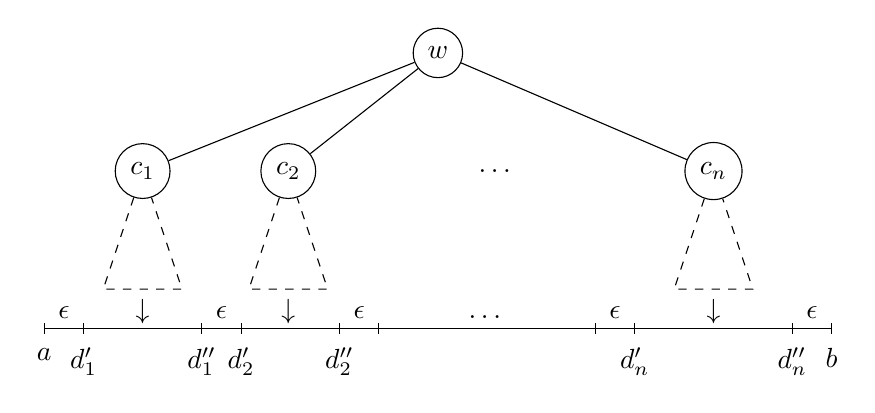
\begin{tikzpicture}[main/.style = {draw, circle}]
      \node [draw=none, label=below:$a$] (a) at (-5, -3.5) {};
      \node [draw=none, label=below:$b$] (b) at (5, -3.5) {};
      \draw (-5,-3.5) -- (5,-3.5);
      \node [draw=none, label=below:$d'_1$] (d1') at (-4.5, -3.5) {};
      \node [draw=none, label=below:$d''_1$] (d1'') at (-3, -3.5) {};
      \node [draw=none, label=below:$d'_2$] (d2') at (-2.5, -3.5) {};
      \node [draw=none, label=below:$d''_2$] (d2'') at (-1.25, -3.5) {};
      \node [draw=none] (d3') at (-.75, -3.5) {};
      \node [draw=none] (dn1'') at (2, -3.5) {};
      \node [draw=none, label=below:$d'_n$] (dn') at (2.5, -3.5) {};
      \node [draw=none, label=below:$d''_n$] (dn'') at (4.5, -3.5) {};
      \draw [draw=none] (a) -- node[midway, above] {$\epsilon$} (d1');
      \draw [draw=none] (d1'') -- node[midway, above] {$\epsilon$} (d2');
      \draw [draw=none] (d2'') -- node[midway, above] {$\epsilon$} (d3');
      \draw [draw=none] (dn1'') -- node[midway, above] {$\epsilon$} (dn');
      \draw [draw=none] (dn'') -- node[midway, above] {$\epsilon$} (b);
      \draw [draw=none] (d2'') -- node[midway, above] {$\dots$} (dn');

      \foreach \n in {a, b, d1', d1'', d2', d2'', d3', dn1'', dn', dn''}
               {
                 \draw ($ (\n) + (0, +2pt) $) -- ($ (\n) - (0, 2pt) $);
               }
      \node [main] (w) {$w$}
        child {node [main, xshift = -1.5cm] (c1) {$c_1$}}
        child {node [main, xshift = -1.15cm] (c2) {$c_2$}}
        child {node {$\dots$} edge from parent [draw=none]}
        child {node [main, xshift = 1.25cm] (cn) {$c_n$}};
        \foreach \n in {c1, c2, cn}
                 {
                   \draw [dashed] (\n) -- +(-.5,-1.5) -- node[midway, below] {$\downarrow$} +(.5,-1.5) -- (\n);
                 }
    \end{tikzpicture}
  \end{figure}

  Let $f_i$ be the preserving tree mapping from the induction hypothesis for $SubTree(T, c_i)$, $\mu \restriction V_{c_i}$ and $d'_{c_i}$ (the interval $[d'_{c_i}, d''_{c_i}]$). Now, we can define $f$:
  \begin{equation*}
    f \eqdef \{ \langle w, p \rangle \} \cup \bigcup_{\mathclap{1 \leq i \leq n}}f_i
  \end{equation*}

  The domains of these functions are disjoint, so $f$ is a function from $V_w$ to $\Pol(\R)$. Clearly $a < d'_i < d''_i < d'_j < d''_j < b$ for $1 \leq i < j \leq n$, so
  \begin{equation*}
    (\forall u \in V_w)(f(u) \subseteq [a, b]).
  \end{equation*}
  Further,
  \begin{equation*}
    \bigcup_{\mathclap{u \in V_w}}f(u) = p \cup \bigcup_{\mathclap{1 \leq i \leq n}} [d'_i, d''_{i}] = [a, b]
  \end{equation*}
  and $a \in p = f(w)$, $b \in p = f(w)$.

  Now it remains to prove that $f$ is a preserving tree mapping.
  \begin{itemize}
  \item To show the parthood property, suppose $u_1 \in V_w$, $u_2 \in V_w$ and $u_1 \neq u_2$.
    \begin{itemize}
    \item If $u_1$ and $u_2$ are both in $V_{c_i}$ for some $i \in \{1, \dots n\}$, given that $f_i$ is a preserving tree mapping, $f(u_1) \bcap f(u_2) = f_i(u_1) \bcap f_i(u_2) = \emptyset$.
    \item If $u_1 \in V_{c_i}$ and $u_2 \in V_{c_j}$, for some $i, j \in \{1, \dots, n\}$ and $i \neq j$, then $f(u_1) = f_i(u_1) \subseteq [d'_i, d''_i]$ and $f(u_2) = f_j(u_2) \subseteq [d'_j, d''_j]$. $[d'_i, d''_i] \cap [d'_j, d''_j] = \emptyset$, so $f(u_1) \bcap f(u_2) \subseteq f(u_1) \cap f(u_2) = \emptyset$.
    \item If $u_1 = w$ or $u_2 = w$, without loss of generality, assume $u_1 = w$. Then $u_2 \in V_i$ for some $i \in \{1, \dots n\}$. Thus, $f(u_1) = p$ and $f(u_2) \subseteq [d'_i, d''_i]$.
      \begin{equation*}
        f(u_1) \bcap f(u_2) \subseteq f(u_1) \cap f(u_2) \subseteq p \cap [d'_i, d''_i] \subseteq \{d'_i, d''_i\}
      \end{equation*}
and so $f(u_1) \bcap f(u_2) = \emptyset$.
    \end{itemize}
  \item To show the contact property, suppose $u_1 \in V_w$, $u_2 \in V_w$ and $u_1 \neq u_2$.
    \begin{itemize}
    \item If $u_1$ and $u_2$ are both in $V_{c_i}$ for some $i \in \{1, \dots n\}$, $f(u_1) = f_i(u_1)$, $f(u_2) = f_i(u_2)$
      \begin{align*}
        \bcont(f(u_1), f(u_1)) &\leftrightarrow \bcont(f_i(u_1), f_i(u_1)) \equivih \\
        \{u_1, u_2\} \in E_{c_i} &\leftrightarrow \{u_1, u_2\} \in E_w.
      \end{align*}
    \item If $u_1 \in V_{c_i}$ and $u_2 \in V_{c_j}$, for some $i, j \in \{1, \dots, n\}$ and $i \neq j$, then $\{u_1, u_1\} \not \in E_w$. $f(u_1) = f_i(u_1) \subseteq [d'_i, d''_i]$, $f(u_2) = f_j(u_2) \subseteq [d'_j, d''_j]$. $[d'_i, d''_i] \cap [d'_j, d''_j] = \emptyset$, so $f(u_1) \cap f(u_2) = \emptyset$ and hence $\bcont(f(u_1), f(u_2))$ does not hold.
    \item If $u_1 = w$ or $u_2 = w$, without loss of generality, assume $u_1 = w$. Then $u_2 \in V_i$ for some $i \in \{1, \dots n\}$.
      \begin{align*}
        \{u_1, u_2\} \in E_w &\leftrightarrow \\
        u_2 = c_i &\equivih \\
        d'_i \in f_i(c_i) \text{ or } d''_i \in f_i(c_i) &\leftrightarrow &(\text{considering the definition of p}) \\
        p \cap f_i(c_i) \neq \emptyset &\leftrightarrow \\
        f(u_1) \cap f(u_2) \neq \emptyset &\leftrightarrow \\
        \bcont(f(u_1), f(u_2))
      \end{align*}
    \end{itemize}
  \item For the measure property, simply note that it holds for $f_i$ and $u \in V_{c_i}$, where $i = 1, \dots, n$, by induction hypothesis and that
    \begin{equation*}
      \mu^\R(f(w)) = \mu^\R(p) \eqdef \epsilon + \epsilon + (n - 1)\epsilon = (n+1) \frac{\mu(w)}{n + 1} = \mu(w).
    \end{equation*}
  \end{itemize}
Finally, note that the given definition of $f$ is easily implemented in a procedure. Thus, $f$ is effectively constructible from $f_1, f_2, \dots, f_n$.
\end{proof}

The result of the lemma is slightly generalized below to allow a different vertex in the tree to touch the right end of the interval.
\begin{lemma}[Tree Mapping to Interval, Arbitrary Right End]
    Let $T = \langle V, E \rangle$ be a rooted tree with root $r$. For any $\mu : V \rightarrow \R^+$, $s \in V$, $a \in \R$ and $b = a + \sum_{u \in V}m(u)$ there is an effective procedure to construct a preserving tree mapping $f$ of $\langle T, \mu \rangle$ such that:
  \begin{itemize}
  \item $\bigcup_{u \in V}f(u) = [a, b]$,
  \item $a \in f(r)$ and $b \in f(s)$.
  \end{itemize}
\end{lemma}
\begin{proof}
  If $r = s$, the previous lemma is directly applied.

  Suppose $r \neq s$ and $v_1, v_2, \dots, v_n = s$ are the vertices along the path from $r$ to $s$. Let
  \begin{equation*}
    \epsilon \eqdef \frac{\min\{v_1, v_2, \dots, v_n\}}{2}.
  \end{equation*}
  Consider the modification to $\mu$:
  \begin{equation*}
    \mu'(u) \eqdef
    \begin{cases}
      \mu(u) - \epsilon & \text{if } u \in \{v_1, v_2, \dots, v_n\} \\
      \mu(u) & \text{otherwise.}
    \end{cases}
  \end{equation*}
  Let $f'$ be the result of the application of the previous lemma to the same tree, but with the function $\mu'$ and for the interval $[a, a + \mu'(V)] = [a, b - n\epsilon]$.
  \begin{equation*}
    f(u) \eqdef
    \begin{cases}
      f'(u) \cup [b - (n - i + 1)\epsilon, b - (n - i)\epsilon] & \text{if } u = v_i, \text{ for } i \in \{1, 2, \dots, n\} \\
      f'(u) & \text{otherwise}
    \end{cases}
  \end{equation*}
  \begin{figure}[ht]
    \centering
    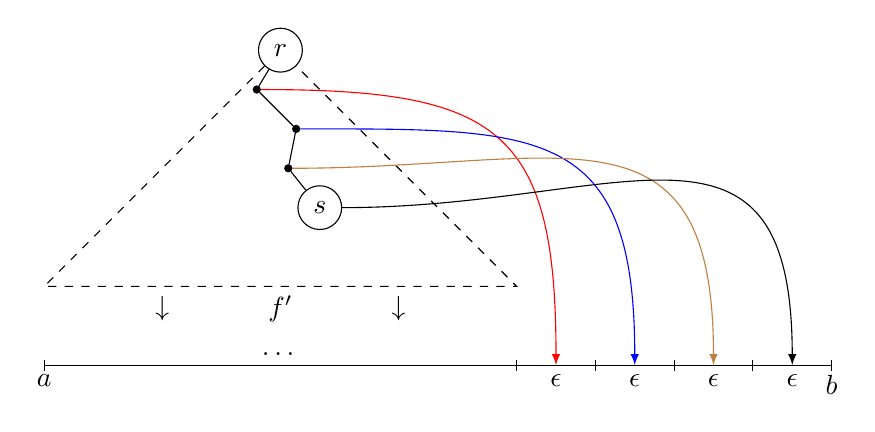
\begin{tikzpicture}[main/.style = {draw, circle}, v/.style = {circle, inner sep = 0pt, outer sep = 0pt, minimum size = 3pt, fill = black}, a/.style = {-latex}]
      \node [main] (r) at (-2, 0) {$r$};
      \node [v] (v1) at (-2.3, -.5) {};
      \node [v] (v2) at (-1.8, -1) {};
      \node [v] (v3) at (-1.9, -1.5) {};
      \node [main] (s) at (-1.5, -2) {$s$};
      \draw [] (r) -- (v1) -- (v2) -- (v3) -- (s);
      \draw [dashed] (r) -- +(-3,-3) -- node[pos=.25, below] {$\downarrow$} node[pos=.5, below] {$f'$} node[pos=.75, below] {$\downarrow$} +(3,-3) -- (r);

      \node [coordinate, label=below:$a$] (a) at (-5, -4) {};
      \node [coordinate, label=below:$b$] (b) at (5, -4) {};
      \draw (a) -- (b);
      \node [coordinate] (1) at (1, -4) {};
      \node [coordinate] (2) at (2, -4) {};
      \node [coordinate] (3) at (3, -4) {};
      \node [coordinate] (4) at (4, -4) {};

      \draw [draw=none] (1) -- node[coordinate, midway, label=below:$\epsilon$] (x1) {} (2);
      \draw [draw=none] (2) -- node[coordinate, midway, label=below:$\epsilon$] (x2) {} (3);
      \draw [draw=none] (3) -- node[coordinate, midway, label=below:$\epsilon$] (x3) {} (4);
      \draw [draw=none] (4) -- node[coordinate, midway, label=below:$\epsilon$] (xs) {} (b);

      \draw [a, red] (v1) to [out=0, in=90, looseness=1.5] (x1);
      \draw [a, blue] (v2) to [out=0, in=90, looseness=1.5] (x2);
      \draw [a, brown] (v3) to [out=0, in=90, looseness=1.5] (x3);
      \draw [a] (s) to [out=0, in=90, looseness=1.5] (xs);

      \draw [draw=none] (a) -- node[midway, above] {$\dots$} (1);

      \foreach \n in {a, b, 1, 2, 3, 4} {
        \draw ($ (\n) + (0, +2pt) $) -- ($ (\n) - (0, 2pt) $);
      }
    \end{tikzpicture}
  \end{figure}

  Clearly, for $1 \leq i < j \leq n$,
  \begin{align*}
    a &< b - n\epsilon \leq \\
    b - (n - i + 1)\epsilon &< b - (n - i)\epsilon \leq \\
    b - (n - j + 1)\epsilon &< b - (n - j)\epsilon \leq b.
  \end{align*}

  It can be seen by direct inspection that
  \begin{align*}
    &\bigcup_{u \in V}f(u) = [a, b], \\
    &a \in f(r) \text{ and } b \in f(s).
  \end{align*}

  \begin{itemize}
  \item To show the parthood and contact properties of $f$ simultaneously, consider $u_1, u_2 \in V$, $u_1 \neq u_2$.
    \begin{itemize}
    \item If both $u_1$ and $u_2$ are not in $\{r, v_1, \dots, v_n\}$, then $f(u_1) = f'(u_1)$ and $f(u_2) = f'(u_2)$ and the properties hold since $f'$ is a preserving tree mapping.
    \item If $u_1 \in \{r, v_1, \dots, v_n\}$, $u_2 \not\in \{r, v_1, \dots, v_n\}$ or vice-versa, then
      \begin{equation*}
        f(u_2) = f'(u_2) \subsetneq [a, b - n\epsilon] \text{, so } f(u_1) \cap f(u_2) \subseteq [a, b - n\epsilon].
      \end{equation*}
      Therefore,
      \begin{align*}
        f(u_1) \cap f(u_2) &= f'(u_1) \cap f'(u_2) \\
        f(u_1) \bcap f(u_2) &= f'(u_1) \bcap f'(u_2)
      \end{align*}
      and again the fact that $f'$ is a preserving tree mapping is used.
    \item If $u_1 = v_i$ and $u_2 = v_j$, without loss of generality, $i < j$.
      \begin{itemize}
      \item If $\{u_1, u_2\} \in E$, then $i + 1 = j$.
        \begin{align*}
          &f(u_1) \bcap f(u_2) \subseteq f(u_1) \cap f(u_2) = \\
          &(f'(u_1) \cap f'(u_2)) \cup \{b - (n - i)\epsilon\}.
        \end{align*}
        $f'(u_1) \cap f'(u_2)$ is finite, so $f(u_1) \bcap f(u_2) = \emptyset$. Also,
        \begin{equation*}
          b - (n - i)\epsilon \in f(u_1) \cap f(u_2) \text{, i.e. } \bcont(f(u_1), f(u_2)).
        \end{equation*}
      \item If $\{u_1, u_2\} \not\in E$, $f'(u_1) \cap f'(u_2) = \emptyset$, because $f'$ is a preserving tree mapping and
        \begin{equation*}
          (f(u_1) \cap f(u_2)) \cap [b - n\epsilon, b] = \emptyset,
        \end{equation*}
        so $f(u_1) \cap f(u_2) = \emptyset$ and of course $f(u_1) \bcap f(u_2) = \emptyset$.
      \end{itemize}
    \item To show the measure property for $u \in V$, consider two simple cases:
      \begin{itemize}
      \item if $u \in \{v_1, \dots, v_n\}$, then
        \begin{align*}
          \mu^\R(f(u)) &= \mu^\R(f'(u)) + \epsilon = \\
          \mu'(u) + \epsilon &= (\mu(u) - \epsilon) + \epsilon = \\
          &= \mu(u);
        \end{align*}
      \item otherwise, $\mu^\R(f(u)) = \mu^\R(f'(u)) = \mu'(u) = \mu(u)$.
      \end{itemize}
    \end{itemize}
  \end{itemize}
\end{proof}

In the lemma below, the same idea is applied to trees with a root of infinite measure and half the real line.

\begin{lemma}[Tree Mapping to Half Line]
    Let $T = \langle V, E \rangle$ be a rooted tree with root $r$. For any $\mu : V \rightarrow \R^+ \cup \{\infty\}$ such that $(\forall v \in V)(\mu(v) = \infty \leftrightarrow v = r)$ and any $a \in \R$ there is an effective procedure to construct a preserving tree mapping $f$ of $\langle T, \mu \rangle$ such that:
  \begin{itemize}
  \item $\bigcup_{u \in V}f(u) = [a, \infty)$,
  \item $a \in f(r)$.
  \end{itemize}
\end{lemma}
\begin{proof}
  Let $c_1, c_2, \dots, c_n$ be the children of $r$. If $n = 0$, the entire mapping is $\{\langle r, [a, \infty) \rangle\}$. If not, let
  \begin{align*}
    a_i &\eqdef a + \sum_{j < i}\left(1 + \mu(SubTree(T, c_j))\right)\\
    b_i &\eqdef a_i + \mu(SubTree(T, c_i)),
  \end{align*} for $i \in \{1, \dots, n\}$. Let
  \begin{equation*}
    p \eqdef [a, a_1] \cup \bigcup_{\mathclap{1 \leq i \leq n}}[b_i, a_{i+1}]
  \end{equation*}

  \begin{figure}[ht]
    \centering
    \begin{tikzpicture}[main/.style = {draw, circle}]
      \node [draw=none, label=below:$a$] (a) at (-5, -3.5) {};
      \draw [-latex] (-5,-3.5) -- (6.5,-3.5);
      \node [draw=none, label=below:$a_1$] (d1') at (-4.5, -3.5) {};
      \node [draw=none, label=below:$b_1$] (d1'') at (-3, -3.5) {};
      \node [draw=none, label=below:$a_2$] (d2') at (-2.5, -3.5) {};
      \node [draw=none, label=below:$b_2$] (d2'') at (-1.25, -3.5) {};
      \node [draw=none] (d3') at (-.75, -3.5) {};
      \node [draw=none] (dn1'') at (2, -3.5) {};
      \node [draw=none, label=below:$a_n$] (dn') at (2.5, -3.5) {};
      \node [draw=none, label=below:$b_n$] (dn'') at (4.5, -3.5) {};
      \draw [draw=none] (a) -- node[midway, above] {$1$} (d1');
      \draw [draw=none] (d1'') -- node[midway, above] {$1$} (d2');
      \draw [draw=none] (d2'') -- node[midway, above] {$1$} (d3');
      \draw [draw=none] (dn1'') -- node[midway, above] {$1$} (dn');
      \draw [draw=none] (d3') -- node[midway, above] {$\dots$} (dn1'');

      \foreach \n in {a, d1', d1'', d2', d2'', d3', dn1'', dn', dn''}
               {
                 \draw ($ (\n) + (0, +2pt) $) -- ($ (\n) - (0, 2pt) $);
               }
      \node [main] (w) {$r$}
        child {node [main, xshift = -1.5cm] (c1) {$c_1$}}
        child {node [main, xshift = -1.15cm] (c2) {$c_2$}}
        child {node {$\dots$} edge from parent [draw=none]}
        child {node [main, xshift = 1.25cm] (cn) {$c_n$}};
        \foreach \n in {c1, c2, cn}
                 {
                   \draw [dashed] (\n) -- +(-.5,-1.5) -- node[midway, below] {$\downarrow$} +(.5,-1.5) -- (\n);
                 }
    \end{tikzpicture}
  \end{figure}

  We apply the (Tree Mapping to Interval, Root at Both Ends) lemma to each child $c_i$ ($i \in \{1, \dots, n\}$) and interval $[a_i, b_i]$ to get $f_1, f_2, \dots, f_n$ and define $f$:
  \begin{equation*}
    f(u) \eqdef
    \begin{cases}
      f_i(u) & \text{if } u \in SubTree(T, c_i), \text{ for some } i \in \{1, \dots, n\} \\
      p      & \text{if } u = r
    \end{cases}
  \end{equation*}

  The rest of the proof is analogous to the induction step of the proof of the (Tree Mapping to Interval, Root at Both Ends) lemma, except for the simplification of the measure of $f(r)$ being $\infty$.
\end{proof}
\begin{corollary}
The same can be done on the interval $(-\infty, a]$ by mirror symmetry.
\end{corollary}

\begin{lemma}[Tree Mapping to the Real Line]
    Let $T = \langle V, E \rangle$ be a tree. Given any $\mu : V \rightarrow \R^+ \cup \{\infty\}$ such that there are exactly two vertices in $V$ with infinite values for $\mu$, there is an effective procedure to construct a preserving tree mapping $f$ of $\langle T, \mu \rangle$ such that $\bigcup_{u \in V}f(u) = (-\infty, \infty)$.
\end{lemma}
\begin{proof}
Let $i_1$ and $i_2$ be those exactly two vertices with infinite values for $\mu$, $\mu(i_1) = \mu(i_2) = \infty$. Let $i_1, w_1, w_2, \dots, w_n, i_2$ be the simple path from $i_1$ to $i_2$. The graph $\langle V, E \setminus \{\{i_1, w_1\}, \{w_n, i_2\}\} \rangle$ has three connected components: one containing $i_1$, one containing $w_1, \dots, w_n$ and one containing $i_2$. Let $\langle V_{i_1}, E_{i_1} \rangle$, $\langle V_w, E_v \rangle$ and $\langle V_{i_2}, E_{i_2} \rangle$ respectively be the trees induced by those components.

  Consider $\langle V_{i_1}, E_{i_1} \rangle$ and $\langle V_{i_2}, E_{i_2} \rangle$ as rooted trees with roots $i_1$ and $i_2$ respectively. They satisfy the conditions for the (Tree Mapping to Half Line) lemma and corollary (with $\mu \restriction V_{i_1}$ and $\mu \restriction V_{i_2}$). Thus, let $f_{i_1}$ be the mapping from the corollary for $\langle V_{i_1}, E_{i_1} \rangle$ and interval $(-\infty, 0]$ and $f_{i_2}$ be the mapping from the lemma for $\langle V_{i_1}, E_{i_1} \rangle$ and interval $[\mu(V_w), \infty)$.

    Now, consider $\langle V_w, E_v \rangle$ as a rooted tree with root $w_1$. The (Tree Mapping to Interval, Arbitrary Right End) lemma is applied to this rooted tree with $w_n$ in the role of the vertex $s$ (and $\mu \restriction V_w$), resulting in a preserving tree mapping $f_w$ onto the interval $[0, \mu(V_w)]$.

    \begin{figure}[ht]
      \centering
      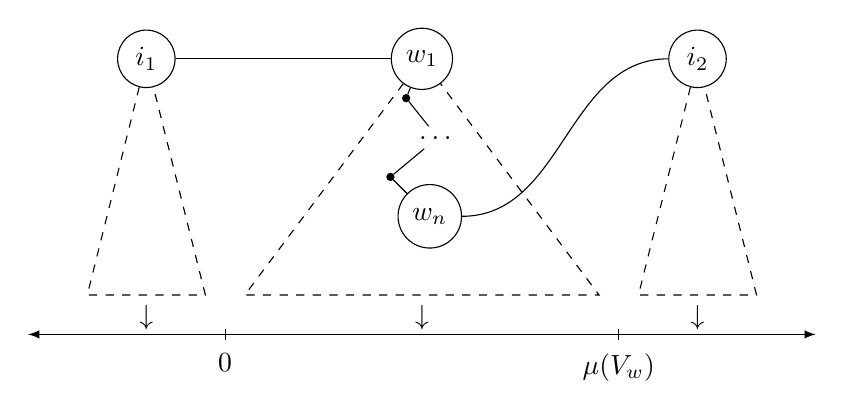
\begin{tikzpicture}[main/.style = {draw, circle}, v/.style = {circle, inner sep = 0pt, outer sep = 0pt, minimum size = 3pt, fill = black}]
        \draw [latex-latex] (-5,-3.5) -- (5,-3.5);

        \node [draw=none, label=below:$0$] (0) at (-2.5, -3.5) {};
        \node [draw=none, label=below:$\mu(V_w)$] (1) at (2.5, -3.5) {};

        \foreach \n in {0, 1}
                 {
                   \draw ($ (\n) + (0, +2pt) $) -- ($ (\n) - (0, 2pt) $);
                 }
                 \node [main] (i1) at (-3.5, 0) {$i_1$};
                 \node [main] (i2) at (3.5, 0) {$i_2$};

                 \node [main] (v1) at (0, 0) {$w_1$};
                 \node [v] (v2) at (-.2, -.5) {};
                 \node [] (v3) at (.2, -1) {$\dots$};
                 \node [v] (v4) at (-.4, -1.5) {};
                 \node [main] (vn) at (.1, -2) {$w_n$};
                 \draw [] (v1) -- (v2) -- (v3) -- (v4) -- (vn);
                 \draw [dashed] (v1) -- +(-2.25,-3) -- node[pos=.5, below] {$\downarrow$} +(2.25,-3) -- (v1);

                 \draw (i1) -- (v1);
                 \draw (vn) to [out=0, in=180, looseness = 1] (i2);
                 \foreach \n in {i1, i2}
                          {
                            \draw [dashed] (\n) -- +(-.75,-3) -- node[midway, below] {$\downarrow$} +(.75,-3) -- (\n);
                          }
      \end{tikzpicture}
    \end{figure}

    It should be noted that if $n = 0$, i.e. $i_1$ and $i_2$ are directly connected by an edge, then there would only be two connected components. In that case, $\langle V_w, E_v \rangle$ would be an empty graph. This poses no problem to the rest of the proof, as then $\mu(V_w) = 0$ and this empty graph would be mapped to $\emptyset$.

    Let $f = f_{i_1} \cup f_w \cup f_{i_2}$. First, it is useful to note that
    \begin{align*}
      & \bigcup_{i \in V}f(i) = \bigcup_{i \in V_{i_1}}f_{i_1}(i) \cup \bigcup_{i \in V_w}f_w(i) \cup \bigcup_{i \in V_{i_2}}f_{i_2}(i) = \\
      & (-\infty, 0] \cup [0, \mu(V_w)] \cup [\mu(V_w), \infty) = \R.
    \end{align*}
    Now follows a proof that $f$ is a preserving tree mapping of $\langle \langle V, E \rangle, \mu \rangle$.
    \begin{itemize}
    \item Let $u_1 \in V$ and $u_2 \in V$, $u_1 \neq u_2$.
      \begin{itemize}
      \item If $u_1$ and $u_2$ are in the same connected component of the disconnected graph, then the parthood and contact properties are satisfied for $f$ since $f_{i_1}$, $f_w$, and $f_{i_2}$ are preserving tree mappings.
      \item If $u_1$ is in one of $V_{i_1}$, $V_{i_2}$ and $u_2$ in the other, then $f(u_1) \subseteq (-\infty, 0]$ and $f(u_2) \subseteq [\mu(V_w), \infty)$ or vice-versa.
    Thus, $f(u_1) \cap f(u_2) \neq \emptyset$ occurs exactly when $\{u_1, u_2\} = \{i_1, i_2\}$ and $\mu(V_w) = 0$. In this case $\{u_1, u_2\} \in E$, so the parthood property holds.

    Either way, $f(u_1) \bcap f(u_2) = \emptyset$, so the contact property also holds.

  \item Suppose $u_1$ is in $V_w$ and $u_2$ in $V_{i_1}$. Then $f(u_1) \subseteq (-\infty, 0]$ and $f(u_2) \subseteq [0, \mu(V_w)]$. Of course, $f(u_1) \bcap f(u_2) = \emptyset$. $f(u_1) \cap f(u_2) \neq \emptyset$ holds by the construction of the lemma exactly if $u_1 = i_1$ and $u_2 = w_1$, in  which case $\{u_1, u_2\} \in E$.

    A similar argument is made if $u_1$ and $u_2$ switch places above or if $u_1$ is in $V_{i_2}$ and $u_2$ is in $V_w$ or the other way around.
      \end{itemize}
    \item For any $u \in V$, $u$ is in one of $V_{i_1}$, $V_w$ or $V_{i_1}$. In all three cases, $\mu^\R(f(u)) = \mu(u)$ since $f_{i_1}$, $f_w$ and $f_{i_2}$ are preserving tree mappings.
    \end{itemize}
\end{proof}

\begin{lemma}[Non-intersecting Interior]
  Let $p$ and $q$ be polytopes. If $p \bcap q = \emptyset$, then $Int(p) \cap q = \emptyset$.
\end{lemma}
\begin{proof}
  For the sake of contradiction, let $x \in Int(p) \cap q$. $x \in Int(p)$, so there is a neighborhood $u_x$ of $x$, such that $u_x \subseteq p$. On the other hand, $x \in q$ and $q = Cl(Int(q))$, so every neighborhood of $x$ intersects $Int(q)$, $u_x$ in particular. Let $y \in u_x \cap Int(q)$. $y \in u_x$ and $u_x \subseteq p$, so $y \in Int(p)$ and so $y \in Int(p) \cap Int(q)$. Therefore \[\emptyset \neq Int(p) \cap Int(q) = Int(p \cap q) \subseteq Cl(Int(p \cap q)) = p \bcap q,\] a contradiction.
\end{proof}

\begin{lemma}[Relational Structure Conversion]
  Let $S = \langle \B^W, \mathcal{C}^\kappa, \leq_\mu \rangle$ be a convertible relational structure and $v$ be a valuation. If $\phi$ is a formula from $\lang$ and $\langle S, v \rangle \models \phi$, then a valuation $v_\R: \Vars \rightarrow \Pol(\R)$ such that $\langle S^\R, v_\R \rangle \models \phi$ can be effectively constructed.
\end{lemma}
\begin{proof}
  $S$ is a convertible relational structure, so by the corollary of the (Untying) lemma, let $S' = \langle \B^{W'}, \mathcal{C}^{\kappa'}, \leq_{\mu'} \rangle$ and $v'$ be a convertible relational structure and a valuation which model the same formulas and it holds that $Gr(S')$ is a tree.

  Since $S'$ is convertible, there are exactly two vertices with infinite values for $\mu$ in the tree $Gr(S')$ and the (Tree Mapping to the Real Line) lemma can be applied to obtain the preserving tree mapping $f$, such that $\bigcup_{u \in V}f(u) = (-\infty, \infty)$.

  Now follows the proof that for any term $\tau$ of $\lang$, \[v_\R(\tau) = \bigcup\{ f(i) \mid i \in v'(\tau)\}.\] Let $v_\R(x) \eqdef \bigcup\{ f(i) \mid i \in v'(x) \}$.

    For variables the statement is true by definition. For the constants:
    \begin{equation*}
      v_\R(0) \eqdef \emptyset = \bigcup\{ f(i) \mid i \in \emptyset\} \eqdef \bigcup\{ f(i) \mid i \in v'(0)\}
    \end{equation*}
    and
    \begin{align*}
      & v_\R(1) \eqdef \R = (-\infty, 0] \cup [0, \mu(V_w)] \cup [\mu(V_w), \infty) = \\
    & \bigcup\{ f(i) \mid i \in V_{i_1}\} \cup \bigcup\{ f(i) \mid i \in V_w\} \cup \bigcup\{ f(i) \mid i \in V_{i_2}\} = \\
    & \bigcup\{ f(i) \mid i \in V\} \eqdef \bigcup\{ f(i) \mid i \in v'(1)\}
    \end{align*}
Suppose that the statement is true for $\tau_1$ and $\tau_2$, terms of $\lang$. For the union operation:
    \begin{align*}
      & v_\R(\tau_1 \lcup \tau_2) \eqdef v_\R(\tau_1) \cup v_\R(\tau_2) \eqih \\
      & \bigcup\{ f(i) \mid i \in v'(\tau_1)\} \cup \bigcup\{ f(i) \mid i \in v'(\tau_2)\} = \\
      & \bigcup\{ f(i) \mid i \in v'(\tau_1 \lcup \tau_2)\}
    \end{align*}
    and for intersection:
    \begin{align*}
      & v_\R(\tau_1 \lcap \tau_2) \eqdef v_\R(\tau_1) \bcap v_\R(\tau_2) \eqih \\
      & \bigcup\left\{ f(i) \mid i \in v'(\tau_1)\right\} \bcap \bigcup\left\{ f(j) \mid j \in v'(\tau_2)\right\} = & (v'(\tau_1) \text{ is finite}) \\
      & \bigcup\left\{ f(i) \bcap \bigcup\left\{ f(j) \mid j \in v'(\tau_2)\right\} \mid i \in v'(\tau_1)\right\} = & (v'(\tau_2) \text{ is finite}) \\
      & \bigcup\left\{ \bigcup\left\{ f(i) \bcap f(j) \mid j \in v'(\tau_2)\right\} \mid i \in v'(\tau_1)\right\} = \\
      & \bigcup\left\{ f(i) \bcap f(j) \mid j \in v'(\tau_2), i \in v'(\tau_1)\right\} = & (i \neq j \rightarrow f(i) \bcap f(j) = \emptyset) \\
      & \bigcup\left\{ f(i) \mid i \in v'(\tau_1) \cap v'(\tau_2)\right\} \eqdef \\
      & \bigcup\left\{ f(i) \mid i \in v'(\tau_1 \lcap \tau_2)\right\}
    \end{align*}
    For complement:
    \begin{align*}
      & v_\R(\tau_1\lstar) \eqdef Cl\left(\R \setminus v_\R(\tau_1)\right) \eqih Cl\left(\R \setminus \bigcup\left\{ f(i) \mid i \in v'(\tau_1)\right\}\right) = \\
      & Cl\left(\bigcup\left\{ f(i) \mid i \in \left(v'(\tau_1) \cup V \setminus v'(\tau_1)\right)\right\} \setminus \bigcup\left\{ f(i) \mid i \in v'(\tau_1)\right\}\right) = \\
      & Cl\left(\bigcup\left\{ f(i) \mid i \in V \setminus v'(\tau_1)\right\} \setminus \bigcup\left\{ f(j) \mid j \in v'(\tau_1)\right\}\right) = \\
      & Cl\left(\bigcup \left\{ f(i) \setminus \bigcup \left\{ f(j) \mid j \in v'(\tau_1) \right\} \mid i \in V \setminus v'(\tau_1)\right\}\right) = \\
      & Cl\left(\bigcup\left\{ \bigcap\left\{ f(i) \setminus f(j) \mid j \in v'(\tau_1)\right\} \mid i \in V \setminus v'(\tau_1)\right\}\right) = & (V \text{ is finite})\\
      & \bigcup\left\{ Cl\left(\bigcap\left\{ f(i) \setminus f(j) \mid j \in v'(\tau_1)\right\}\right) \mid i \in V \setminus v'(\tau_1)\right\} = & (*)\\
      & \bigcup\left\{ f(i) \mid i \in V \setminus v'(\tau_1)\right\} = \\
      & \bigcup\left\{ f(i) \mid i \in v'(\tau_1\lstar)\right\}
    \end{align*}

    To show that $(*)$ holds, it needs to be shown that \[Cl\left(\bigcap\left\{ f(i) \setminus f(j) \mid j \in v'(\tau_1)\right\}\right) = f(i).\]

    To do that, consider that if $i \in V \setminus v'(\tau_1)$ and $j \in v'(\tau_1)$, then $i \neq j$. Thus, $f(i) \bcap f(j) = \emptyset$. Given this, $Int(f(i)) \cap f(j) = \emptyset$, as shown in non-intersecting interior lemma.

    Therefore, $Int(f(i)) \subseteq f(i) \setminus f(j)$. From here, \[Int(f(i)) \subseteq \bigcap\{ f(i) \setminus f(j) \mid j \in v'(\tau_1)\}\] and applying $Cl$ to both sides, \[Cl(Int(f(i))) \subseteq Cl\left(\bigcap \{ f(i) \setminus f(j) \mid j \in v'(\tau_1)\}\right)\] is obtained. $f(i) = Cl(Int(f(i)))$, so \[f(i) \subseteq Cl\left(\bigcap\{ f(i) \setminus f(j) \mid j \in v'(\tau_1)\}\right).\]

    On the other hand, \[Cl\left(\bigcap\{ f(i) \setminus f(j) \mid j \in v'(\tau_1)\}\right) \subseteq Cl\left(\bigcap\{ f(i) \mid j \in v'(\tau_1)\}\right) = f(i)\] Thus, \[f(i) = Cl\left(\bigcap\{ f(i) \setminus f(j) \mid j \in v'(\tau_1)\}\right).\]

    To finish the proof of the lemma, a proof by induction on the construction of $\phi$ that $\langle S^\R, v_\R \rangle \models \phi \leftrightarrow \langle S', v' \rangle \models \phi$ follows.
    \begin{itemize}
    \item For $\bot$ and $\top$, the statement is trivial.
    \item For $\tau_1 \lpart \tau_2$,
      \begin{align*}
        \langle S^\R, v_\R \rangle \models \tau_1 \lpart \tau_2 &\leftrightarrow \\
        v_\R(\tau_1) \subseteq v_\R(\tau_2) &\leftrightarrow \\
        \bigcup\{f(i) \mid i \in v'(\tau_1)\} \subseteq \bigcup\{f(i) \mid i \in v'(\tau_2)\} &\leftrightarrow & (*) \\
        v'(\tau_1) \subseteq v'(\tau_2) &\leftrightarrow \\
        \langle S', v' \rangle \models \tau_1 \lpart \tau_2
      \end{align*}
      The equivalence at $(*)$ from right to left is direct. From left to right, let $i \in v'(\tau_1)$. \[Int(f(i)) \subseteq f(i) \subseteq \bigcup\{f(i) \mid i \in v'(\tau_1)\} \subseteq \bigcup\{f(i) \mid i \in v'(\tau_2)\}.\] Using again the non-intersecting interior lemma, $Int(f(i)) \cap f(j) = \emptyset$ for $i \neq j$, so $i \in v'(\tau_2)$ must hold to allow $Int(f(i)) \subseteq \bigcup\{f(i) \mid i \in v'(\tau_2)\}$. Thus, $v'(\tau_1) \subseteq v'(\tau_2)$.
    \item For $\lcont(\tau_1, \tau_2)$,
      \begin{align*}
        \langle S^\R, v_\R \rangle \models \lcont(\tau_1, \tau_2) &\leftrightarrow \\
        v_\R(\tau_1) \cap v_\R(\tau_2) \neq \emptyset &\leftrightarrow \\
        \bigcup\{f(i) \mid i \in v'(\tau_1)\} \cap \bigcup\{f(i) \mid i \in v'(\tau_2)\} \neq \emptyset &\leftrightarrow \\
        (\exists i \in v'(\tau_1))(\exists j \in v'(\tau_2))(f(i) \cap f(j) \neq \emptyset) &\leftrightarrow \\
        (\exists i \in v'(\tau_1))(\exists j \in v'(\tau_2))(\bcont(f(i), f(j))) &\leftrightarrow \\
        (\exists i \in v'(\tau_1))(\exists j \in v'(\tau_2))(\{i, j\} \in E) &\leftrightarrow \\
        \langle S', v' \rangle \models \lcont(\tau_1, \tau_2)
      \end{align*}
    \item For $\tau_1 \lmeasure \tau_2$,
      \begin{align*}
        \langle S^\R, v_\R \rangle \models \tau_1 \lmeasure \tau_2 &\leftrightarrow \\
        \mu^\R(v_\R(\tau_1)) \leq \mu^\R(v_\R(\tau_2)) &\leftrightarrow \\
        \mu^\R\left(\bigcup\{f(i) \mid i \in v'(\tau_1)\}\right) \leq \mu^\R\left(\bigcup\{f(i) \mid i \in v'(\tau_2)\}\right) &\leftrightarrow (*) \\
        \sum_{\mathclap{i \in v'(\tau_1)}}\mu^\R(f(i)) \leq \sum_{\mathclap{i \in v'(\tau_2)}}\mu^\R(f(i)) &\leftrightarrow \\
        \sum_{\mathclap{i \in v'(\tau_1)}}\mu(i) \leq \sum_{\mathclap{i \in v'(\tau_2)}}\mu(i) &\leftrightarrow \\
        \langle S', v' \rangle \models \tau_1 \lmeasure \tau_2
      \end{align*}
      $(*)$ is by additivity of $\mu^\R$ in $\B^\R$.
    \end{itemize}
\end{proof}
\section{Axiomatization}
This section presents a decidable set of formulas of $\lang$ which axiomatize $S^\R$. That is to say they are valid in $S^\R$ and all formulas of $\lang$, valid in $S^\R$, can be formally derived from them.

Formal derivation is meant in the usual proof-theoretic sense. The logical axioms and rules of inference can for example be in Hilbert style for a first order language with equality. In the case of $\lang$, where no quantifiers are present, logical axioms or rules relating to quantifiers are superfluous and could be left out.

The axioms that pertain to $\lcup$, $\lcap$ and $\lstar$ are those of a Boolean algebra and are given below. The particular set chosen here is as in (TODO: cite Halmos).
\begin{tasks}(2)
\task[] (B1) $x \lcap 1 \lparteq x$
\task[] (B2) $x \lcup 0 \lparteq x$
\task[] (B3) $x \lcap x\lstar \lparteq 0$
\task[] (B4) $x \lcup x\lstar \lparteq 1$
\task[] (B5) $x \lcap y \lparteq y \lcap x$
\task[] (B6) $x \lcup y \lparteq y \lcup x$
\task[] (B7) $x \lcap (y \lcup z) \lparteq (x \lcap y) \lcup (x \lcap z)$
\task[] (B8) $x \lcup (y \lcap z) \lparteq (x \lcup y) \lcap (x \lcup z)$
\end{tasks}
It will be assumed without further mention that basic statements about Boolean algebras can be formally derived from these and that these formal proofs can be effectively generated. The parthood relation is the partial ordering of the Boolean algebra. Formal equality occurs when two objects are parts of each other.
\begin{tasks}(2)
  \task[] (B9) $(x \lpart y) \Leftrightarrow (x \lcap y \lparteq x)$
  \task[] (B10) $(x \lparteq y) \Leftrightarrow (x \lpart y \land y \lpart x)$
\end{tasks}

The axioms for contact are:
\begin{tasks}(1)
  \task[] (C1) $(x \not \lparteq 0) \Leftrightarrow \lcont(x, x)$
  \task[] (C2) $\lcont(x, y \lcup z) \Leftrightarrow \lcont(x, y) \lor \lcont(x, z)$
  \task[] (C3) $\lcont(x, y) \Rightarrow \lcont(y, x)$
  \task[] (C4) $(x \not \lparteq 0) \land (x \not \lparteq 1) \Rightarrow \lcont(x, x\lstar)$
\end{tasks}

The axioms for measure are infinitely many. The finite portion is:
\begin{tasks}(1)
  \task[] (M1) $(x \lmeasure y) \land (y \lcap z \lparteq 0) \Rightarrow (x \lcup z) \lmeasure (y \lcup z)$
  \task[] (M2) $(x \lcap z \lparteq 0) \land (y \lcap z \lparteq 0) \land (z \lmeasures 1) \Rightarrow (x \lmeasure y \Leftrightarrow (x \lcup z) \lmeasure (y \lcup z))$
  \task[] (M3) $(x \lcap z \lparteq 0) \land (y \lcap z \lparteq 0) \land (z \lmeasures 1) \Rightarrow (x \lmeasures y \Leftrightarrow (x \lcup z) \lmeasures (y \lcup z))$
  \task[] (M4) $(x \lmeasureeq 1) \lor (x\lstar \lmeasureeq 1)$
  \task[] (M5) $\lnot(x \lmeasureeq 1 \land y \lmeasureeq 1 \land z \lmeasureeq 1 \land (x \lcap y \lparteq 0) \land (x \lcap z \lparteq 0) \land (y \lcap z \lparteq 0))$
  \task[] (M6) $(x \lmeasureeq 0) \Leftrightarrow (x \lparteq 0)$
\end{tasks}

%\begin{equation*}
%  (x \lcup y \lcup z \lparteq 1) \land (x \lmeasureeq 1) \land (y \lmeasures 1) %\land (z \lmeasureeq 1) \land \lcont(x \lcup y, z) \rightarrow \lcont(x, z)
%\end{equation*}

The rest of the measure axioms form an infinite, but decidable set and are presented below.
\begin{definition}[$(n, \leq)$-type and $(n, <)$-type inequalities]
  Let $r_1, r_2, \dots, r_n$ be variables for real numbers and $I' \subseteq \{1, 2, \dots, n\}$, $I'' \subseteq \{1, 2, \dots, n\}$. Then
  \begin{equation*}
    \sum_{i \in I'}r_i \leq \sum_{i \in I''}r_i
  \end{equation*}
  is an \emph{$(n, \leq)$-type inequality} and
  \begin{equation*}
    \sum_{i \in I'}r_i < \sum_{i \in I''}r_i
  \end{equation*}
  is an \emph{$(n, <)$-type inequality}.
\end{definition}
Note that $\sum_{i \in \emptyset}r_i \eqdef 0$ by convention.

\begin{definition}[$R_n$ System of Inequalities]
  Any system of $(n, \leq)$- and $(n, <)$-type inequalities over the same variables $r_1, r_2, \dots, r_n$, which also contains the inequalities $0 \leq r_i$, for all $i \in {1, 2, \dots, n}$, is called an \emph{$R_n$ system}.
\end{definition}
\begin{definition}[Formula $\phi_R$, Matched to $R_n$ System]
  Let $R$ be an $R_n$ system. To any $(n, \leq)$-type inequality
  \begin{equation*}
    \sum_{i \in I'}r_i \leq \sum_{i \in I''}r_i,
  \end{equation*}
  the formula of $\lang$
  \begin{equation*}
    \bigsqcup_{i \in I'}x_i \lmeasure \bigsqcup_{i \in I''}x_i
  \end{equation*}
  is matched. Analogously, to any $(n, <)$-type inequality
  \begin{equation*}
    \sum_{i \in I'}r_i < \sum_{i \in I''}r_i,
  \end{equation*}
  the formula of $\lang$
  \begin{equation*}
    \bigsqcup_{i \in I'}x_i \lmeasures \bigsqcup_{i \in I''}x_i
  \end{equation*}
  is matched.

  The conjunction of all formulas matched to $(n, \leq)$- and $(n, <)$-type inequalities of $R$ is denoted by $\phi_R$, the formula matched to $R$.
\end{definition}

Given these definitions, the rest of the axioms that concern the qualitative measure can be defined. For every natural number $n$, for every $R_n$ system $R$, if $R$ does not have a solution in which exactly one or exactly two variables are assigned values of $\infty$, then
\[
\text{(M}_R\text{)} \left(\bigwedge_{1 \leq i < j \leq n} (x_i \lcap x_j \lparteq 0) \land \bigsqcup_{\mathclap{1 \leq i \leq n}} x_i \lparteq 1\right) \Rightarrow \lnot \phi_R
\]
is an axiom.
\subsection{Decidability}
The axioms described above are infinitely many. This raises the question of their decidability, particularly the axioms (M$_R$), which form the infinite part.

\begin{proposition}
  There exists an effective procedure to determine if any system with $n$ real variables (not allowing $\infty$), containing non-strict and strict linear inequalities with real coefficients, i.e.
  \[
  \begin{array}{|l@{}}
    \begin{aligned}
      &a_{1, 1}r_1 + a_{1, 2}r_2 + \dots + a_{1, n}r_n &&\leq b_1 \\
      &a_{2, 1}r_1 + a_{2, 2}r_2 + \dots + a_{2, n}r_n &&\leq b_2 \\
      &\dots&&\dots \\
      &a_{m, 1}r_1 + a_{m, 2}r_2 + \dots + a_{m, n}r_n &&\leq b_m \\
      &a_{m+1, 1}r_1 + a_{m+1, 2}r_2 + \dots + a_{m+1, n}r_n &&< b_{m+1} \\
      &a_{m+2, 1}r_1 + a_{m+2, 2}r_2 + \dots + a_{m+2, n}r_n &&< b_{m+2} \\
      &\dots&&\dots \\
      &a_{m+k, 1}r_1 + a_{m+k, 2}r_2 + \dots + a_{m+k, n}r_n &&< b_{m+k}
    \end{aligned}
  \end{array}
  \]
  has a solution and if so, to produce that solution.
\end{proposition}
\begin{proof}
  After rearrangement of the inequalities to leave $r_n$ on the left side,
  \[
  \begin{array}{|l@{}}
    \begin{aligned}
      &r_n \;\; \leq\!\!\mathbig{/}\!\!\geq && - \frac{a_{1, 1}}{a_{1,n}}r_1 - \frac{a_{1, 2}}{a_{1, n}}r_2 - \dots - \frac{a_{1, n - 1}}{a_{1, n}}r_{n - 1} + \frac{b_1}{a_{1, n}} \\
      &r_n \;\; \leq\!\!\mathbig{/}\!\!\geq && - \frac{a_{2, 1}}{a_{2,n}}r_1 - \frac{a_{2, 2}}{a_{2, n}}r_2 - \dots - \frac{a_{2, n - 1}}{a_{2, n}}r_{n - 1} + \frac{b_2}{a_{2, n}} \\
      &\dots&&\dots \\
      &r_n \;\; \leq\!\!\mathbig{/}\!\!\geq && - \frac{a_{m, 1}}{a_{m,n}}r_1 - \frac{a_{m, 2}}{a_{m, n}}r_2 - \dots - \frac{a_{m, n - 1}}{a_{m, n}}r_{n - 1} + \frac{b_m}{a_{m, n}} \\
      &r_n \;\; <\!\!\mathbig{/}\!\!> && - \frac{a_{m+1, 1}}{a_{m+1,n}}r_1 - \frac{a_{m+1, 2}}{a_{m+1, n}}r_2 - \dots - \frac{a_{m+1, n - 1}}{a_{m+1, n}}r_{n - 1} + \frac{b_{m+1}}{a_{m+1, n}} \\
      &r_n \;\; <\!\!\mathbig{/}\!\!> && - \frac{a_{m+2, 1}}{a_{m+2,n}}r_1 - \frac{a_{m+2, 2}}{a_{m+2, n}}r_2 - \dots - \frac{a_{m+2, n - 1}}{a_{m+2, n}}r_{n - 1} + \frac{b_{m+2}}{a_{m+2, n}} \\
      &\dots&&\dots \\
      &r_n \;\; <\!\!\mathbig{/}\!\!> && - \frac{a_{m+k, 1}}{a_{m+k,n}}r_1 - \frac{a_{m+k, 2}}{a_{m+k, n}}r_2 - \dots - \frac{a_{m+k, n - 1}}{a_{m+k, n}}r_{n - 1} + \frac{b_{m+k}}{a_{m+k, n}} \\
    \end{aligned}
  \end{array}
  \]
  is obtained, where $\leq\!\!\mathbig{/}\!\!\geq$ stands for $\leq$ or $\geq$ and $<\!\!\mathbig{/}\!\!>$ stands for $<$ or $>$, depending on the sign of $a_{i, n}$, for $i = 1, \dots, m+k$. Thus, for any assignment to $r_1, r_2, \dots, r_{n-1}$, a series of strict and non-strict upper and lower bounds on $r_n$ are achieved.

  Given this, the rest of the proof will be by induction on the number of variables.

  Suppose $n = 1$. The strict and non-strict upper and lower bounds on the single variable $r_1$ are fully determined and do not depend on any further variable assignments. If two lower bounds or two upper bounds are equal, one strict and one non-strict, then the strict one implies the non-strict one, so the non-strict is superfluous and is ignored. Let $L$ be the set of lower bounds and $U$ be the set of upper bounds. If $\max L = \min U$, and these two bounds are non-strict, then $\max L$ is a solution for $r_1$. Additionally, if $\max L < \min U$, then any value in $(L_g, U_l)$ is a solution, for example $(L_g + U_l)/2$. In the other cases, there is no solution.

  Suppose $n > 1$. For each right-hand side (linear expression) of the transformed system that forms a lower bound $l$ and each each right-hand side that forms an upper bound $u$, consider the inequality $U \leq L$, if both bounds are non-strict and $U < L$, if at least one of them is strict. Thus, a new system of these linear inequalities is constructed for the $n-1$ variables $r_1, r_2, \dots, r_{n-1}$. By induction hypothesis, there is a procedure to find a solution to this system or to conclude that there is none.

  This new system is a consequence of the first, so if it has no solution, then the initial system also has no solution. On the other hand, if $\rho_1, \rho_2, \dots, \rho_{n-1}$ is a solution for $r_1, r_2, \dots, r_{n-1}$ in the new system, let $L_\rho$ and $U_\rho$ be the sets of upper and lower bounds on $r_n$, achieved by substituting $r_i$ for $\rho_i$ in the previous system, where $i = 1, 2, \dots, n-1$. Again, as in the base case, superfluous non-strict bounds are ignored.

  If $\max L_\rho = \min U_\rho$, then both bounds are non-strict (if they were strict, $\rho_1, \rho_2, \dots, \rho_{n-1}$ wouldn't be a solution) and assigning $\max L_\rho$ to $r_n$ yields a solution for the original system. Otherwise, assigning any value in the interval $(\max L_\rho, \min U_\rho)$ to $r_n$ yields a solution, for example $(\max L_\rho + \min U_\rho)/2$.
\end{proof}
\begin{corollary}
  There exists an effective procedure to determine if any $R_n$ system $R$ has a solution where exactly one or exactly two variables are assigned $\infty$ and if so, to produce that solution.
\end{corollary}
\begin{proof}
  There are finitely many possible choices for exactly one or exactly two variables of those in $R$ to be assigned $\infty$. For any such assignment, a new system is obtained. If a solution is found for any these new systems, it yields a solution to $R$ and otherwise $R$ has no solution (in which exactly one or exactly two variables are assigned $\infty$).

  For any inequality of this new system, the following cases are considered:
  \begin{itemize}
  \item when the inequality is strict,
    \begin{itemize}
    \item if an infinite assignment features on the left side, the system has no solution;
    \item if an infinite assignment features on the right side, but not on the left, the inequality can be ignored;
    \item if no infinite assignment features in the inequality, no change is made;
    \end{itemize}
  \item when the inequality is non-strict,
    \begin{itemize}
    \item if an infinite assignment features on the right side, the inequality can be ignored;
    \item if an infinite assignment features on the left side, but not on the right, the system has no solution;
    \item if no infinite assignment features in the inequality, no change is made.
    \end{itemize}
  \end{itemize}
  If after this consideration, it has not been established that the system has no solution, then the inequalities which feature $\infty$ have been eliminated and the obtained system is of linear strict and non-strict inequalities. Therefore, the statement from the proposition can be applied.
\end{proof}

\begin{proposition}
  There is an effective procedure to decide if any formula $\phi$ of $\lang$ is an axiom.
\end{proposition}
\begin{proof}
  First, check if $\phi$ is any of the finitely many axioms (B1) - (B10), (C1) - (C4) or (M1) - (M6). If not, what remains is to check whether it is (M$_R$), for some $R_n$ system $R$.

  If there are $k$ variables in $\phi$, then $\phi$ can correspond only to an $R_k$ system. There are finitely many $R_k$ systems so it remains only to exhaustively check for each one of them if:
  \begin{itemize}
  \item it has a solution with exactly one or exactly two variables assigned to $\infty$,
  \item $\phi$ corresponds to that system.
  \end{itemize}
  If both are true for some $R_k$ system, then $\phi$ is an axiom. Otherwise it isn't.
\end{proof}

\begin{proposition}[Correctness]
  All axioms are valid in $S^\R$.
\end{proposition}
\begin{proof}
  The axioms (B1) - (B10) are valid in $S^\R$, since $\B^\R$ is a Boolean algebra and the validity of axioms (C1)-(C3) is trivial.

  (C4) Suppose $p \in \Pol(\R)$, $p \neq \emptyset$ and $p \neq \R$. Since $p \neq \emptyset$, the standard representation $C_p$ of $p$ is non-empty. Let $b \in C_p$. Since $p \neq \R$, $b \neq \R$ and so let $x$ be any finite endpoint of $b$. $x$ is a point of closure of $p$ and also of $\R \setminus p$, thus $x \in p \bcap p \bstar$.

  (M1) Suppose that $p$, $q$ and $r$ are polytopes, $q \bcap r = \emptyset$ and also $\mu^\R(p) \leq \mu^\R(q)$. Using the properties of the Lebesgue measure, \[\mu^\R(p \cup r) \leq \mu^\R(p) + \mu^\R(r) \leq \mu^\R(q) + \mu^\R(r) = \mu^\R(q \cup r).\]
  Therefore $p \cup r \bmeasure q \cup r$.

  (M2) Suppose that $p$, $q$ and $r$ are polytopes, $p \bcap r = \emptyset$, $q \bcap r = \emptyset$ and $\mu^\R(r) \neq \infty$.
  \begin{align*}
    p &\bmeasure q &&\leftrightarrow \\
    \mu^\R(p) &\leq \mu^\R(q) &&\leftrightarrow & (\mu^\R(r) \neq \infty)\\
    \mu^\R(p) + \mu^\R(r) &\leq \mu^\R(q) + \mu^\R(r) &&\leftrightarrow \\
    \mu^\R(p \cup r) &\leq \mu^\R(q \cup r) &&\leftrightarrow \\
    p \cup r &\bmeasure q \cup r &&\leftrightarrow
  \end{align*}

  (M3) is analogous to (M2).

  (M4) Let $p \in \Pol(\R)$ and suppose $\mu^\R(p) \neq \infty$. Then all basis polytopes in the standard representation of $p$ have only finite endpoints. Let $x$ be the greatest right endpoint. $[x, \infty) \subseteq p\bstar$, so $\mu^\R(p\bstar) = \infty$.

    (M5) Suppose for the sake of contradiction that $p$, $q$ and $r$ are polytopes, $\mu^\R(p) = \infty$, $\mu^\R(q) = \infty$, $\mu^\R(r) = \infty$, $p \bcap q = \emptyset$, $p \bcap r = \emptyset$ and $q \bcap r = \emptyset$.
    Since $\mu^\R(p) = \infty$, there must be basis polytope $b$ in the standard representation of $p$, such that $\mu^\R(b) = \infty$. Then, $b$ must have an infinite endpoint. Without loss of generality, suppose that endpoint is $\infty$. If $q$ or $r$ have a basis interval in their standard representation with an endpoint of $\infty$, then $p \cap q \neq \emptyset$ or $p \cap r \neq \emptyset$.

    However, by the same argument, $q$ and $r$ each must have at least one basis interval with an infinite endpoint in their standard representations. As shown, that endpoint is not $\infty$, so it must be $-\infty$. This means that $q \cap r \neq \emptyset$, a contradiction.

    (M6) is a direct consequence of the proposition that the only polytope with measure 0 is $\emptyset$, which is given in the section defining polytopes.

    (M$_R$) Let $R$ be an $R_n$ system with no solution in which exactly one or exactly two of the variables are assigned values of $\infty$. Let $p_1, p_2, \dots, p_n$ be polytopes, such that $\bigcup_{i = 1, 2, \dots, n}p_i = \R$ and for all $i = 1, 2, \dots, n$ and $j = 1, 2, \dots, n$, if $i \neq j$, then $p_i \bcap p_j = \emptyset$.

    By additivity, it must be that $\mu^\R(p_i) = \infty$, for some $i = 1, 2, \dots, n$. Further, if for some distinct $i = 1, 2, \dots, n$, $j = 1, 2, \dots, n$ and $k = 1, 2, \dots, n$ it holds that $\mu^\R(p_i) = \infty$, $\mu^\R(p_j) = \infty$ and $\mu^\R(p_k) = \infty$, then this would contradict axiom (M5). Therefore, there are exactly one or exactly two polytopes among $p_1, p_2, \dots, p_n$, with infinite measures.

    Suppose for the sake of contradiction, that $\phi_\R$ (with individual variables substituted for the corresponding polytopes among $p_1, p_2, \dots, p_n$) holds. Consider the following assignment to the variables $r_1, r_2, \dots, r_n$ of $R$: $r_i = \mu^\R(p_i)$.

    Any subformula of $\phi_R$, matched to an $(n, \leq)$-type inequality yields that
    \[
        \bigsqcup_{i \in I'}p_i \bmeasure \bigsqcup_{i \in I''}p_i,
        \] for the appropriate $I'$ and $I''$.

        Therefore, using additivity of the measure \[
        \sum_{\mathclap{i \in I'}}\mu^\R(p_i) \leq \sum_{\mathclap{i \in I''}}\mu^\R(p_i),
        \]
        which means that the corresponding $(n, \leq)$-type inequality holds.

        An analogous argument can be made for $(n, <)$-type inequalities and their corresponding subformulas. Clearly $0 \leq \mu^\R(p_i)$ for all $i = 1, 2, \dots, n$.

        Therefore, all inequalities of $R$ are satisfied and $R$ has a solution with exactly one or exactly two variables assigned to $\infty$, a contradiction.
\end{proof}
\subsection{Completeness}
\end{document}
